%%%%%%%%%%%%%%%%%%%%%%%%%%%%%%%%%%%%%%%%%%%%%%%%%%%%%%%%%%%%%%%%%%%%%%%%%
%%%%%%%%%%%%%%%%%%%%%%%%%%%%%%%%%%%%%%%%%%%%%%%%%%%%%%%%%%%%%%%%%%%%%%%%%
\part{Functions and Data}

%%%%%%%%%%%%%%%%%%%%%%%%%%%%%%%%%%%%%%%%%%%%%%%%%%%%%%%%%%%%%%%%%%%%%%%%

\chapter{Polynomial and Spline Interpolation}

%%%%%%%%%%%%%%%%%%%%%%%%%%%%%

\subsection*{A Chemical Reaction}

In a chemical reaction the concentration level $y$ of
the product at time $t$ was measured every half hour.
The following results were found:\\
\begin{tabular}{c|ccccc}
t & 0 & .5 & 1.0 & 1.5 & 2.0 \\ \hline
y & 0 & .19 & .26 & .29 & .31
\end{tabular}

We can input this data into \textsc{Matlab} as
\begin{lstlisting}[frame=none,numbers=left]
t1 = 0:.5:2
y1 = [ 0 .19 .26 .29 .31 ]
\end{lstlisting}
and plot the data with
\begin{lstlisting}[frame=none,numbers=left]
plot(t1,y1)
\end{lstlisting}
\textsc{Matlab} automatically connects the data with line segments, so the graph has corners.
%
What if we want a smoother graph? Try
\begin{lstlisting}[frame=none,numbers=left]
plot(t1,y1,'*')
\end{lstlisting}
which will produce just asterisks at the data points.  Next click on
\verb&Tools&, then click on the \verb&Basic Fitting& option.  This
should produce a small window with several fitting options.  Begin
clicking them one at a time, clicking them off before clicking the
next. Which ones produce a good-looking fit?  You should note that the
spline, the shape-preserving interpolant, and the 4th degree polynomial
produce very good curves. The others do not.  


%%%%%%%%%%%%%%%%%%%%%%%%%%%%%

\subsection*{Polynomial Interpolation}

Suppose we have \(n\) data points \(\{(x_i,y_i)\}_{i=1}^n\).
A interpolant is a function \(f(x)\) such that 
\(y_i=f(x_i)\) for \(i=1,\dots,n\).
%
The most general  polynomial with degree $d$ is
$$
    p_d(x) = a_d x^d + a_{d-1} x^{d-1} + \ldots + a_1 x + a_0\,,
$$
which has \(d+1\) coefficients.
A polynomial interpolant with degree $d$ thus must satisfy
$$
    y_i=p_d(x_i) = a_d x_i^d + a_{d-1} x_i^{d-1} + \ldots + a_1 x_i +
    a_0
\quad\text{for \(i=1,\dots,n\).}
$$
This system is a linear system in the unknowns $a_0, \ldots, a_n$ and
{\em solving linear systems is what
computers do best}.
If \(n=d+1\),
then the system of equations has \(n\)
equations and \(n\)
unknowns, so in general there is a unique solution.
This is the case in the example above:
there are 5 data points so there is exactly one 4th degree polynomial
that interpolates the data.

If \(n < d+1\) then the system is underdetermined and so in general
will have an infinite number of solutions. 
When we tried to use a 5th or higher degree polynomial above,
\textsc{Matlab} returned a warning that the polynomial
is not unique since ``degree $>=$
number of data points''.

If the data \(\{(x_i,y_i)\}_{i=1}^n\) has repeated \(x\)-values with
distinct \(y\)-values, then the system of equations is inconsistent
and there will be no solution.
%
If \(n > d+1\) then the system has more equations than unknowns, so it
is overdetermined and in general will have no solution. 
%
In these cases \textsc{Matlab} does produce a function, but it does
not satisfy  \(p(x_i)=y_i\) for \(i=1,\dots,n\) and so is not an interpolant. 
Instead it is a least-squares fit, which we will study in
Lecture~\ref{sec:leastsquares}.


%%%%%%%%%%%%%%%%%%%%%%%%%

\subsection*{Predicting the future?}

Suppose we want to use the data to extrapolate into the future.
Set the plot to the 4th degree polynomial. Then click the \verb&Edit&
button and select the \verb&Axes Properties& option.
A box should appear that allows you to adjust the domain of the $x$
axes. Change the upper limit of the $x$-axis from $2$ to $4$.
Based on the 4th degree polynomial, what will the chemical reaction
do in the future? Is this reasonable?

Next change from 4th degree polynomial to spline interpolant.
According to the spline, what will the chemical reaction do
in the future? Try the shape-preserving interpolant also.

From our (limited) knowledge of chemical reactions, what
should be the behavior as time goes on? It should reach
a limiting value (chemical equilibrium). Could we use the
data to predict this equilibrium value? Yes, we could
and it is done all the time in many different contexts,
but to do so we need to know that there is an equilibrium
to predict. This requires that we understand the chemistry
of the problem. Thus we have the following principle:
To {\em extrapolate} beyond the data, one must have some
knowledge of the process.


%%%%%%%%%%%%%%%%%%%%%%%%%%%%%

\subsection*{More data}

Generally one would think that more data is better. Input the
following data vectors:
\begin{lstlisting}[frame=none,numbers=left]
t2 = [ 0  .1  .4  .5  .6  1.0  1.4 1.5 1.6 1.9 2.0]
y2 = [ 0  .06 .17 .19 .21 .26  .29 .29 .30 .31 .31]
\end{lstlisting}
There are 11 data points, so a 10-th degree polynomial will
fit the data. However, this does not give a good graph. Thus:
{\bf Polynomial interpolation is better for small data sets.}



%%%%%%%%%%%%%%%%%%%%%%%%%%%%%

\subsection*{A challenging data set}

Input the following data set:
\begin{lstlisting}[frame=none,numbers=left]
x = -4:1:5
y = [ 0 0 0 1 1 1 0 0 0 0]
\end{lstlisting}
and plot it:
\begin{lstlisting}[frame=none,numbers=left]
plot(x,y,'*')
\end{lstlisting}
There are 10 data points, so there is a unique 9 degree polynomial that
fits the data. Under \verb&Tools& and \verb&Basic Fitting& select the
9th degree polynomial fit. How does it look?  De-select the
9th degree polynomial and select the spline interpolant. This should
produce a much more satisfactory graph and the shape-preserving
spline should be even better. 
%In this section we learn whata spline is.


%%%%%%%%%%%%%%%%%%%%%%%%%%%%%

\subsection*{The idea of a spline}

The general idea of a spline is this: on each interval between data
points, represent the graph with a simple function.
The simplest spline is something very familiar to you;
it is obtained by connecting the data with lines.
Since linear is the most simple function of all,
linear interpolation is the simplest form of spline. The next simplest
function is quadratic. If we put a quadratic function on each interval
then we should be able to make the graph a lot smoother. If we were
really careful then we should be able to make the curve smooth at
the data points themselves by matching up the derivatives.
This can be done and the result is called a quadratic spline.
Using cubic functions or 4th degree functions should be smoother still.
So, where should we stop? There is an almost universal consensus that
{\em cubic} is the optimal degree for splines and so we focus the
rest of the lecture on cubic splines.



%%%%%%%%%%%%%%%%%%%%%%%%%%%%%

\subsection*{Cubic spline}


Again, the basic idea of the cubic spline is that we represent
the function by a different cubic function on each interval
between data points. That is, if there are $n$ data points, then
the spline $S(x)$ is the function
\begin{equation*}
S(x) = \left\{ \begin{array}{ll}
               C_1(x),    & \quad x_0 \le x \le x_1 \\
               C_i(x),    & \quad x_{i-1} \le x \le x_i \\
               C_n(x), & \quad x_{n-1} \le x \le x_n
               \end{array} \right.
\end{equation*}
where each $C_i$ is a cubic function. The most general cubic
function has the form
$$
    C_i(x) = a_i + b_i x + c_i x^2 + d_i x^3.
$$
To determine the spline we must determine the coefficients, $a_i$,
$b_i$, $c_i$, and $d_i$ for each $i$. Since there are $n$ intervals,
there are $4n$ coefficients to determine.
First we require that the spline interpolate by requiring
\begin{equation*}
C_i(x_{i-1}) = y_{i-1}  \quad \text{and} \quad C_i(x_i) = y_i,
\end{equation*}
at every data point. In other words,
$$
a_i + b_i x_{i-1} + c_i x_{i-1}^2 + d_i x_{i-1}^3 = y_{i-1} \quad \text{and} \quad
a_i + b_i x_i + c_i x_i^2 + d_i x_i^3 = y_i.
$$
Notice that there are $2n$ of these conditions. Then to make $S(x)$ as
smooth as possible we require
\begin{equation*}
\begin{split}
C'_i(x_i) &= C'_{i+1}(x_i)\quad\text{and} \\
C''_i(x_i) &= C''_{i+1}(x_i)
\end{split}
\end{equation*}
at all the internal points, i.e. $x_1$, $x_2, x_3, \ldots, x_{n-1}$.
In terms of the points these conditions can be written as
\begin{equation*}
\begin{split}
b_i + 2 c_i x_i + 3 d_i x_i^2
               &= b_{i+1} + 2 c_{i+1} x_i + 3 d_{i+1} x_i^2 \quad\text{and}\\
 2 c_i  + 6 d_i x_i
               &= 2 c_{i+1}  + 6 d_{i+1} x_i.
\end{split}
\end{equation*}
There are $2(n-1)$ of these conditions. Since each $C_i$ is
cubic, there are a total of $4n$ coefficients in the formula
for $S(x)$. So far we have $4n - 2$ equations, so we are 2 equations short
of being able to determine all the coefficients. At this point we
have to make a choice. The usual choice is to require
\begin{equation*}
     C''_1(x_0) = C''_n(x_n) = 0.
\end{equation*}
These are called {\em natural} or {\em simple} boundary conditions.
The other common option is called {\em clamped} boundary conditions:
\begin{equation*}
     C'_1(x_0) = C'_n(x_n) = 0.
\end{equation*}
The terminology used here is obviously parallel to that used
for beams. That is not the only parallel between beams and
cubic splines. It is an interesting fact that a cubic spline is
exactly the shape of a (linear) beam restrained to match the
data by simple supports.

Note that the equations above are all linear equations
with respect to the unknowns (coefficients). This feature
makes splines easy to calculate since {\em solving linear systems is what
computers do best.}



%%%%%%%%%%%%%%%%%%%%%%%

\subsection*{Exercises}
\begin{list}
{\arabic{chapter}.\arabic{exercise}}{\usecounter{exercise}}

\item You are given the following data:
\begin{lstlisting}[frame=none,numbers=left]
t = [ 0  .1  .499  .5  .6  1.0  1.4 1.5 1.899 1.9 2.0 ]
y = [ 0  .06 .17   .19 .21 .26  .29 .29 .30   .31 .31 ]
\end{lstlisting}
\begin{enumerate}
\item[(a)] Plot the data, using \verb&'*'& at the data points, then try a polynomial fit of the correct degree
  to interpolate this number of data points. 
  \begin{itemize}
  	\item What do you observe?
  	Look closely at the data and identify the points that force the interpolating polynomial to have large derivative.
  	\item What would happen if the \verb*|t| value of $1.899$ was rounded to $1.9$?
  	Is the problem of converting this data to its interpolating polynomial {\em well conditioned} or {\em badly conditioned}?
  \end{itemize}
  
   
  % Give an explanation of this error, in particular why is the term {\em badly conditioned} used?
\item[(b)] Plot the data along with a spline interpolant.  How
  does this compare with the plot above?  What is a way to make the
  plot better?
\end{enumerate}
\end{list}

%%%%%%%%%%%%%%%%%%%%%%%%%%%%%%%%%%%%%%%%%%%%%%%%%%%%%%%%

\chapter{Least Squares Fitting:  Noisy Data}
\label{sec:leastsquares}

Suppose we have \(n\) data points \(\{(x_i,y_i)\}_{i=1}^n\).
In the previous section we learned about interpolation, where the
fitting function \(f(x)\) is required to satisfy  
\(y_i=f(x_i)\) for \(i=1,\dots,n\).
%
Very often  data has a significant amount of noise, so it makes more
sense to only ask for \(y_i\approx f(x_i)\).
The least squares fitting method produces such an \(f\). 
The next illustration shows the effects
noise can have and how least squares is used.

%%%%%%%%%%%%%%%

\subsection*{Traffic flow model}

Suppose you are interested in the time it takes to travel on a certain
section of highway for the sake of planning. According to theory,
assuming up to a moderate amount of traffic, the time should be
approximately
$$
     T(x) = ax + b
$$
where $b$ is the travel time when there is no other traffic and $x$ is
the current number of cars on the road (in hundreds). To determine the
coefficients $a$ and $b$ you could run several experiments which consist
of driving the highway at different times of day and also estimating the number
of cars on the road using a counter. Of course both of these measurements
will contain {\em noise}, i.e.\ random fluctuations.

We could simulate such data in \textsc{Matlab} as follows:
\begin{lstlisting}[frame=none,numbers=left]
x = 1:.1:6;
T = .1*x + 1;
Tn = T + .1*randn(size(x));
plot(x,Tn,'.')
\end{lstlisting}
The data should look like it lies on a line, but with noise.
Click on the \verb&Tools& button and choose \verb&Basic fitting&.
Then choose a \verb&linear& fit. The resulting line should go through the
data in what looks like a very reasonable way. Click on \verb&show equations&.
Compare the equation with $T(x) = .1 x + 1$. The coefficients should
be pretty close considering the amount of noise in the plot.
Next, try to fit the data with a spline. The result should be ugly.
We can see from this example that {\bf splines are not suited to noisy data}.

How does \textsc{Matlab} obtain a very nice line to approximate noisy
data?  The answer is a very standard numerical/statistical method
known as {\em least squares}.


%%%%%%%%%%%%%%%
\subsection*{Least squares}

The least squares method requires you to first select what type of
\(f\) to consider (sometimes called a model) and what parameters it
depends on. For example, you might choose
\[
f(x) = a_1 \exp({a_2 x})+a_0 \quad\text{or}\quad f(x) = a_2 x^2 + a_1 x +a_0\,.  
\]
Given data \(\{(x_i,y_i)\}_{i=1}^n\), we can then determine the error
at each point as \(e_i = y_i - f(x_i)\). 
To make $f$ reasonable,
we wish to simultaneously minimize all the errors $\{e_1,e_2, \ldots, e_n\}$.
There are many possible ways one could go about this, but the standard one
is to try to minimize the {\em sum of the squares} of the errors. That is,
we denote by $\mathcal{E}$ the sum of the squares
\[
\mathcal{E} = \sum_{i=1}^n e_i^2
    = \sum_{i=1}^n \left( y_i - f(x_i) \right)^2
\,.
\]
Since \(f\) depends on some parameters, $\mathcal{E}$ is a function of
those parameters.
To minimize $\mathcal{E}$, we can compute the partial derivatives of
it with respect to each of the parameters, set the results
equal to zero, and solve the resulting system of equations.

%%%%%%%%%%%%%%%
\subsubsection*{Linear least squares}

If we choose \(f\) to depend linearly on the parameters, then the
resulting system of equations will be a linear system, which is easy
to solve. This does not mean we have to choose \(f\) to be a line.
For example, the function \(f(x) = a_2 x^2 + a_1 x +a_0\) is a
quadratic in \(x\), but
depends linearly on each of \(a_2\), \(a_1\), and \(a_0\).
To illustrate the linear least squares process, we will go through it
using this quadratic \(f\).

The error is 
\[
\mathcal{E}(a_0,a_1,a_2) =\sum_{i=1}^n \left( y_i - (a_2 x_i^2 + a_1 x_i +a_0) \right)^2
\,,
\]
which has partial derivatives
\begin{align*}
  \frac{ \partial \mathcal{E}}{\partial a_0} 
  & = -2 \sum_{i=1}^n \left( y_i - (a_2 x_i^2 + a_1 x_i +a_0) \right)\,,\\
  \frac{ \partial \mathcal{E}}{\partial a_1} 
  & = -2 \sum_{i=1}^n \left( y_i - (a_2 x_i^2 + a_1 x_i +a_0) \right)x_i\,,\quad\text{and}\\
  \frac{ \partial \mathcal{E}}{\partial a_2}                                              
  & = -2 \sum_{i=1}^n \left( y_i - (a_2 x_i^2 + a_1 x_i +a_0) \right)x_i^2
    \,.
\end{align*}
Setting these equal to zero and rearranging yields the linear system
\[
\begin{pmatrix}
   \displaystyle\sum_{i=1}^n 1 &  \displaystyle\sum_{i=1}^n x_i &
   \displaystyle\sum_{i=1}^n x_i^2\\
   \displaystyle\sum_{i=1}^n x_i &  \displaystyle\sum_{i=1}^n x_i^2&
   \displaystyle\sum_{i=1}^n x_i^3\\
   \displaystyle\sum_{i=1}^n x_i^2&  \displaystyle\sum_{i=1}^n x_i^3&
   \displaystyle\sum_{i=1}^n x_i^4\\
\end{pmatrix}
\begin{pmatrix}
  a_0 \\ a_1 \\ a_2
\end{pmatrix}
=
\begin{pmatrix}
  \displaystyle\sum_{i=1}^n y_i \\ \displaystyle\sum_{i=1}^n y_ix_i \\ \displaystyle\sum_{i=1}^n y_i x_i^2
\end{pmatrix}
\,.
\]
The entries in the matrix are determined from simple formulas using
the data. Since this is a linear system, it is easily solved.
The process is quick and easily automated, which is one
reason it is very standard.
\textsc{Matlab}'s  basic fitting tool uses this process to obtain a
$d$ degree polynomial fit whenever the number of data points is more than
$d+1$.


\hide{
Consider in the previous example that we wish to fit a line to a lot of data
that does not exactly lie on a line. For the equation of the line we have
only two free coefficients, but we have many data points. We can not possibly
make the line go through every data point, we can only wish for it to come
reasonably close to as many data points as possible. Thus, our line must
have an error with respect to each data point. If $\ell(x)$ is our line
and $\{(x_i,y_i)\}$ are the data, then
$$
      e_i = y_i - \ell(x_i)
$$
is the error of $\ell$ with respect to each $(x_i,y_i)$.
To make $\ell(x)$ reasonable,
we wish to simultaneously minimize all the errors: $\{e_1,e_2, \ldots, e_n\}$.
There are many possible ways one could go about this, but the standard one
is to try to minimize the {\em sum of the squares} of the errors. That is,
we denote by $\mathcal{E}$ the sum of the squares:
\begin{equation}
    \mathcal{E} = \sum_{i=1}^n \left( y_i - \ell(x_i) \right)^2
                = \sum_{i=1}^n \left( y_i - a x_i - b \right)^2 .
\end{equation}
In the above expression $x_i$ and $y_i$ are given, but we are free
to choose $a$ and $b$, so we can think of $\mathcal{E}$ as a function
of $a$ and $b$, i.e. $\mathcal{E}(a,b)$.
In calculus, when one wishes to find a minimum value
of a function of two variables, we set the partial derivatives equal to
zero:
\begin{equation}
\begin{split}
      \frac{ \partial \mathcal{E}}{\partial a} & =
          -2 \sum_{i=1}^n \left( y_i - a x_i -b \right) x_i = 0 \\
 \frac{ \partial \mathcal{E}}{\partial b} & =
          -2 \sum_{i=1}^n \left( y_i - a x_i -b \right) = 0 .
\end{split}
\end{equation}
We can simplify these equations to obtain
\begin{equation}
\begin{split}
\left( \sum_{i=1}^n x_i^2 \right) a + \left( \sum_{i=1}^n x_i \right) b
          &= \sum_{i=1}^n x_i y_i \quad\text{and}\\
 \left( \sum_{i=1}^n x_i \right) a + n b &= \sum_{i=1}^n y_i .
\end{split}
\end{equation}
Thus, the whole problem reduces to a 2 by 2 linear system to find the
coefficients $a$ and $b$. The entries in the matrix are determined from
simple formulas using the data. The process is quick and easily automated,
which is one reason it is very standard.

We could use the same process to obtain a quadratic or higher polynomial
fit to data. If we try to fit an $n$ degree polynomial, the software
has to solve an $n \times n$  linear system, which is easily done.
}

%%%%%%%%%%%%

\subsection*{Drag coefficients}

Drag due to air resistance is proportional to the square of the
velocity, i.e.~$d= kv^2$.  In a wind tunnel experiment the velocity
$v$ can be varied by setting the speed of the fan and the drag can be
measured directly (it is the force on the object).  In this and every
experiment some random noise will occur. The following sequence of
commands replicates the data one might receive from a wind tunnel:
\begin{lstlisting}[frame=none,numbers=left]
v = 0:1:60;
d = .1234*v.^2;
dn = d + .4*v.*randn(size(v));
plot(v,dn,'*')
\end{lstlisting}
The plot should look like a quadratic, but with some noise.  Using the
tools menu, add a quadratic fit and enable the ``show equations''
option.  What is the coefficient of $x^2$? How close is it to 
$0.1234$?

Note that whenever you select a polynomial in \textsc{Matlab}
with a degree less than $n-1$ \textsc{Matlab} will produce a least squares
fit.

You will notice that the quadratic fit includes both a constant and
linear term.  We know from the physical situation that these should
not be there; they are remnants of noise and the fitting
process. Since we know the curve should be $k v^2$, we can do better
by employing that knowledge. For instance, we know that the graph of
$d$ versus $v^2$ should be a straight line. We can produce this easily:
\begin{lstlisting}[frame=none,numbers=left]
z = v.^2;
plot(z,dn,'*')
\end{lstlisting}
By changing the independent variable from $v$ to $z=v^2$ we produced a
plot that looks like a line with noise. Add a linear fit. What is the
linear coefficient? This should be closer to $0.1234$ than using a
quadratic fit.

The second fit still has a constant term, which we know should not be
there.  If there was no noise, then at every data point we would have
$k = d/v^2$. We can express this as a linear system \verb&z'*k = dn'&,
which is badly overdetermined since there are more equations than
unknowns. Since there is noise, each point will give a different
estimate for $k$. In other words, the overdetermined linear system is
also inconsistent. When \textsc{Matlab} encounters such systems, it
automatically gives a least squares solution of the matrix problem,
i.e.~one that minimizes the sum of the squared errors, which is
exactly what we want. To get the least squares estimate for $k$, do
\begin{lstlisting}[frame=none,numbers=left]
k = z'\dn'
\end{lstlisting}
This will produce a number close to .1234.

Note that this is an application where we have physical knowledge. In this
situation extrapolation would be meaningful. For instance we could use
the plot to find the predicted drag at 80 mph.


%%%%%%%%%%%%%
\newpage
\subsection*{Exercises}
\begin{list}
{\arabic{chapter}.\arabic{exercise}}{\usecounter{exercise}}


\item Find two tables of data in an engineering textbook or
  engineering website. Plot each (with \verb&'*'& at data points) and decide if the data is best
  represented by a polynomial interpolant, spline interpolant, or
  least squares fit polynomial.  Label the axes and include a title.
  Turn in the best plot of each.
  Indicate the source and meaning of the data.


\item
  The following table contains information from a chemistry experiment
  in which the concentration of a product was measured at one minute
  intervals:

  \begin{tabular}{c|cccccccc}
    Time & 0     & 1     & 2     & 3     & 4     & 5     & 6     & 7 \\
    \hline
    Concentration & 3.033 & 3.306 & 3.672 & 3.929 & 4.123 & 4.282 & 4.399 & 4.527
  \end{tabular}

  Plot this data. Suppose it is known that this chemical
  reaction should follow the law: $c = a - b \exp(-0.2 t)$. Following
  the example in the notes about the drag coefficients, change
  one of the variables so that the law is a linear function. Then
  plot the new variables and use the linear fit option to estimate
  $a$ and $b$. What will be the eventual concentration? Finally,
  plot the graph of $a - b \exp(-0.2 t)$ on the interval [0,15] (as a
  solid curve), along with the data from the table (using \verb&'*'&).
\end{list}



%%%%%%%%%%%%%%%%%%%%%%%%%%%%%%%%%%%%%%%%%%%%%%%%%%%%%%%%%%%

\chapter{Integration: Left, Right and Trapezoid Rules}
\label{sec:LRTrules}

%%%%%%%%%%%%%%%%%%%%%%%%%%%%%

\subsection*{The Left and Right endpoint rules}

In this section, we wish to approximate a definite integral
$$
\int_a^b f(x) \, dx
\,,
$$
where $f(x)$ is a continuous function.
In calculus we learned that integrals are (signed) areas and can be approximated
by sums of smaller areas, such as the areas of rectangles.
We begin by choosing points $\{x_i\}$  that subdivide $[a,b]$:
$$
a = x_0 < x_1 < \ldots < x_{n-1} < x_n = b.
$$
The subintervals $[x_{i-1}, x_i]$ determine the width $\Delta x_i$ of
each of the approximating
rectangles. For the height, we learned that we can choose any height
of the function $f(x^*_i)$ where $x^*_i \in [x_{i-1},x_i]$. The
resulting approximation is
$$
  \int_a^b f(x) \, dx \approx \sum_{i=1}^n f(x^*_i) \Delta x_i.
$$
To use this to approximate integrals with actual numbers, we
need to have a specific $x^*_i$ in each interval. The two simplest
(and worst) ways to choose $x^*_i$ are as the left-hand point or the
right-hand point of each interval. This gives concrete approximations
which we denote by $L_n$ and $R_n$ given by
\begin{align*}
L_n &= \sum_{i=1}^n f(x_{i-1}) \Delta x_i
\quad\text{and}&
R_n &= \sum_{i=1}^n f(x_i) \Delta x_i
\,.
\end{align*}
\begin{lstlisting}
function L = myleftsum(x,y)
    % produces the left sum from data input.
    % Inputs: x -- vector of the x coordinates of the partition
    %         y -- vector of the corresponding y coordinates
    % Output: returns the approximate integral
    n = length(x);
    L = 0;
    for i = 1:n-1
       % accumulate height times width
       L = L + y(i)*(x(i+1) - x(i));
    end
end
\end{lstlisting}


Often we can take $\{x_i\}$ to be {\em evenly spaced}, with each
interval having the same width:
$$
 h   = \frac{b-a}{n} ,
$$
where $n$ is the number of subintervals. If this is the case, then $L_n$
and $R_n$ simplify to
\begin{align}
\label{evenleft}
L_n  &= h \sum_{i=0}^{n-1} f(x_i)
\quad\text{and}\\
\label{evenright}
R_n &= h \sum_{i=1}^n f(x_i).
\end{align}


The foolishness of choosing left or right endpoints is illustrated
in Figure~\ref{LnRn}. As you can see, for a very simple function like
$f(x) = 1 + .5 x$, each rectangle of $L_n$ is too short, while
each rectangle of $R_n$ is too tall. This will hold for any increasing
function. For decreasing functions $L_n$ will always be too large while
$R_n$ will always be too small.
\begin{figure}
\begin{center}
\setlength{\unitlength}{1 mm}
\begin{picture}(35,50)(0,-1)
	\put(0,0){\vector(1,0){35}}
	\put(0,0){\vector(0,1){49}}
	\put(-2,31){\line(2,1){36}}
%
	\put(0,32){\line(1,0){16}}
	\put(16,0){\line(0,1){40}}
	\put(16,40){\line(1,0){16}}
	\put(32,0){\line(0,1){48}}
\end{picture}
\hspace{2cm}
\begin{picture}(35,50)(0,-1)
	\put(0,0){\vector(1,0){35}}
	\put(0,0){\vector(0,1){49}}
	\put(-2,31){\line(2,1){36}}
%
	\put(0,40){\line(1,0){16}}
	\put(16,0){\line(0,1){48}}
	\put(16,48){\line(1,0){16}}
	\put(32,0){\line(0,1){48}}
\end{picture}
\end{center}
\caption{The left and right sums, $L_n$ and $R_n$.}
\label{LnRn}
\end{figure}

%%%%%%%%%%%%%%%%%%%%%%%%%%%%%

\subsection*{The Trapezoid rule}

Knowing that the errors of $L_n$ and $R_n$ are of opposite sign, a very
reasonable way to get a better approximation is to take an average of
the two. We will call the new approximation $T_n$:
$$
 T_n = \frac{L_n + R_n}{2}.
$$
This method also has a straight-forward geometric interpretation.
On each subrectangle we are using
$$
   A_i = \frac{f(x_{i-1}) + f(x_i)}{2} \Delta x_i
\,,
$$
which is exactly the area of the {\em trapezoid} with sides $f(x_{i-1})$
and $f(x_i)$. We thus call the method the trapezoid method. See
Figure~\ref{trap}.
\begin{figure}[h]
\begin{center}
\setlength{\unitlength}{1 mm}
\begin{picture}(70,60)(0,-1)
	\put(0,0){\vector(1,0){70}}
	\put(0,0){\vector(0,1){59}}
	\qbezier(0,16)(18,-7)(32,32)
	\qbezier(32,32)(46,71)(64,48)
%
	\put(16,0){\line(0,1){8}}
	\put(32,0){\line(0,1){32}}
	\put(48,0){\line(0,1){56}}
	\put(64,0){\line(0,1){48}}
%
	\put(0,16){\line(2,-1){16}}
	\put(32,32){\line(-2,-3){16}}
	\put(32,32){\line(2,3){16}}
	\put(64,48){\line(-2,1){16}}
\end{picture}
\end{center}
\caption{The trapezoid rule, $T_n$.}
\label{trap}
\end{figure}
We can rewrite $T_n$ as
$$
T_n = \sum_{i=1}^n \frac{f(x_{i-1}) + f(x_i)}{2} \Delta x_i .
$$
In the evenly spaced case, we can write this as
\begin{equation}\label{eventrap}
T_n = \frac{h}{2} \bigl( f(x_0) + 2f(x_1) +
                         \ldots + 2f(x_{n-1}) + f(x_n) \bigr).
\end{equation}

{\bf Caution:} The convention used here is to begin numbering
the points at $0$, i.e.~$x_0 = a$; this allows $n$ to be the
number of subintervals and the index of the last point $x_n$.
However, \textsc{Matlab}'s indexing convention
begins at $1$. Thus, when programming in \textsc{Matlab}, the first entry in
\verb&x& will be $x_0$, i.e.~\verb&x(1)&$= x_0$ and \verb&x(n+1)&$=x_n$.


If we are given data about the function, rather than a formula for the
function, often the data are not evenly spaced.  The following
function program could then be used.
\begin{lstlisting}
function T = mytrap(x,y)
    % Calculates the Trapezoid rule approximation of the integral from data
    % Inputs: x -- vector of the x coordinates of the partitian
    %         y -- vector of the corresponding y coordinates
    % Output: returns the approximate integral
    n = length(x);
    T = 0;
    for i = 1:n-1
       % accumulate twice the signed area of the trapezoids
       T = T + (y(i) + y(i+1)) * (x(i+1) - x(i));
    end
    T = T/2; % correct for the missing 1/2
end
\end{lstlisting}


%%%%%%%%%%%%%%%%%%%%%%%%%%%%%

\subsection*{Using the Trapezoid rule for areas in the plane}

Multi-variable Calculus tells us that you
can calculate the area of a region $R$ in the plane by calculating
the line integral
\begin{equation}\label{areaint}
   A = - \oint_{C} y \, dx\,,
\end{equation}
where $C$ is the counter-clockwise curve around the boundary of the region.
We can represent such a curve by consecutive points on it, i.e.~
$\bar{x} = (x_0, x_1, x_2, \ldots, x_{n-1}, x_n)$, and
$\bar{y} = (y_0, y_1, y_2, \ldots, y_{n-1}, y_n)$. Since we are
assuming the curve ends where it begins, we require $(x_n,y_n) = (x_0,y_0)$.
Applying the trapezoid method to the integral (\ref{areaint}) gives
$$
    A = - \sum_{i=1}^n \frac{y_{i-1} + y_i}{2} \, (x_i -x_{i-1})\,.
$$
This formula then is the basis for calculating areas when coordinates
of boundary points are known, but not necessarily formulas for the boundaries
such as in a land survey.

In the following script, we can use this method to approximate the
area of a unit circle using $n$ points on the circle:
\begin{lstlisting}
% Calculates pi using a trapezoid approximation of the unit circle.
format long
n = 10;        % evaluate points on the circle
t = linspace(0,2*pi,n+1);
x = cos(t);
y = sin(t);
plot(x,y)
A = 0      % accumulate (twice) the trapezoid area
for i = 1:n
    A = A - (y(i)+y(i+1))*(x(i+1)-x(i));
end
A = A/2 % correct for the missing 1/2
\end{lstlisting}


%%%%%%%%%%%%%%%%%%%%%%%%%%%%%

\subsection*{Vector Operations using Slicing and Summing}

In the programs above we used loops to explicitly accumulate sums. 
For example, in \verb&mytrap& we had
\begin{lstlisting}
T = 0;
for i = 1:n-1
   T = T + .5*(y(i)+y(i+1))*(x(i+1) - x(i));
end
\end{lstlisting}
The alternative is to use vector operations by taking slices out of
the vectors and using the \verb&sum& function. We can replace the above
code by
\begin{lstlisting}
T = .5*sum( (y(1:n-1)+y(2:n)) .* (x(2:n)-x(1:n-1)) );
\end{lstlisting}
Generally, explicit loops are easier to understand but vector
operations are more efficient and compact.


%%%%%%%%%%%%%

\subsection*{Exercises}
\begin{list}
{\arabic{chapter}.\arabic{exercise}}{\usecounter{exercise}}

\item \label{exr:L4R4} For the integral $\int_1^2 \sqrt{x} \, dx$
  calculate $L_4$, $R_4$, and $T_4$ with even spacing (by hand, but
  use a calculator and a lot of digits) using formulas (\ref{evenleft}), (\ref{evenright})
  and (\ref{eventrap}).  Find the percentage error of these
  approximations, using the exact value.


\item Write a well-commented \textsc{Matlab} {\bf function} program
  \verb&myints& whose inputs are $f$, $a$, $b$ and $n$ and whose
  outputs are $L$, $R$ and $T$, the left, right and trapezoid integral
  approximations for $f$ on $[a,b]$ with $n$ subintervals. To make it
  efficient, 
  \begin{itemize}
  \item take advantage of the fact that $\Delta x_i$ is constant,
  \item use \verb&x = linspace(a,b,n+1)& to make the $x$ values,
  \item use \verb&y = f(x)& to make the $y$ values, 
  \item use slice and \verb&sum& to add the $2$nd to $n$th $y$ entries once,
  \item and then add on the missing
  terms to obtain the left, right and trapezoid approximations.  
  \end{itemize}
  Change to \verb&format long& and apply your program to the integral
  $\int_1^2 \sqrt{x} \, dx$. Compare with the results of the previous
  exercise. Also find $L_{100}$, $R_{100}$ and $T_{100}$ and the
  percentage errors of these approximations.

  Turn in the program and a brief summary of the results.
\end{list}

%%%%%%%%%%%%%%%%%%%%%%%%%%%%%%%%%%%%%%%%%%%%%%%%%%%%%%%%%%%%%%%%%

\chapter{Integration: Midpoint and Simpson's Rules}
\label{sec:MSrules}


%%%%%%%%%%%%%%%%%%%%%%%%%%%%%

\subsection*{Midpoint rule}

If we use the endpoints of the subintervals to approximate the
integral, we run the risk that the values at the endpoints do not
accurately represent the average value of the function on the
subinterval. A point which is much more likely to be close to the
average would be the midpoint of each subinterval.  Using the midpoint
in the sum is called the {\em midpoint rule}. On the $i$-th interval
$[x_{i-1},x_i]$ we will call the midpoint $\bar{x}_i$, i.e.
$$
        \bar{x}_i = \frac{ x_{i-1} + x_i}{2}.
$$
If $\Delta x_i = x_i - x_{i-1}$ is the length of each interval, then using
midpoints to approximate the integral would give the formula
$$
   M_n = \sum_{i=1}^n f(\bar{x}_i) \Delta x_i
\,.
$$
For even spacing, $\Delta x_i = h = (b-a)/n$, and the formula is
\begin{equation}\label{evenmid}
   M_n = h \, \sum_{i=1}^{n} f(\bar{x}_i)
             = h \, (\hat{y}_1 + \hat{y}_2 + \ldots + \hat{y}_n),
\end{equation}
where we define $\hat{y}_i = f(\bar{x}_i)$.

While the midpoint method is obviously better than $L_n$ or $R_n$, it
is not obvious that it is actually better than the trapezoid method $T_n$,
but it is.


%%%%%%%%%%%%%%%%%%%%%%%%%%%%%

\subsection*{Simpson's rule}

Consider Figure~\ref{trapsim}.
\begin{figure}[h]
\begin{center}
\setlength{\unitlength}{1 mm}
\begin{picture}(70,50)(0,-1)
	\put(0,0){\vector(1,0){70}}
	\put(0,0){\vector(0,1){49}}
	\qbezier(-1,10)(40,10)(65,43.5)
%
	\put(32,-1){\line(0,1){2}}
	\put(32,16.5){\circle*{2}}
	\put(64,0){\line(0,1){42}}
	\put(0,10){\line(2,1){64}}
	\put(0,16.5){\line(1,0){64}}
\end{picture}
\end{center}
\caption{Comparing the trapezoid and midpoint method on a single
         subinterval. The function is concave up, in which
         case $T_n$ is too high, while $M_n$ is too low.}
\label{trapsim}
\end{figure}
If $f$ is not linear on a subinterval, then
it can be seen that the errors for the midpoint and trapezoid rules behave
in a very predictable way, they have opposite sign. For example, if the
function is concave up then $T_n$ will be too high, while $M_n$ will be too
low. Thus it makes sense that a better estimate would be to average $T_n$ and
$M_n$. However, in this case we can do better than a simple average. The
error will be minimized if we use a weighted average. To find the proper
weight we take advantage of the fact that for a quadratic function the
errors $EM_n$ and $ET_n$ are exactly related by
$$
     |EM_n| = \frac{1}{2} |ET_n|
\,.
$$
Thus we take the following weighted average of the two, which is called
Simpson's rule:
$$
     S_{2n} = \frac{2}{3} M_n + \frac{1}{3} T_n
\,.
$$
If we use this weighting on a quadratic function the two errors will exactly
cancel.


Notice that we write the subscript as $2n$. That is because we usually think
of $2n$ subintervals in the approximation; the $n$ subintervals of the
trapezoid are further subdivided by the midpoints. We can then number
all the points using integers. If we number them this way we notice
that the number of subintervals must be an even number.

The formula for Simpson's rule if the subintervals are evenly spaced
is the following (with $n$ intervals, where $n$ is even):
$$
   S_n =  \frac{h}{3} \left( f(x_0) + 4f(x_1) + 2f(x_2) + 4f(x_3) +
            \ldots + 2f(x_{n-2}) + 4f(x_{n-1}) + f(x_n) \right)
\,.
$$

Note that if we are presented with data $\{x_i,y_i\}$ where the $x_i$
points are evenly spaced with $x_{i+1} - x_i = \Delta x$, it is easy
to apply Simpson's method:
\begin{equation}\label{datasimp}
   S_n = \frac{h}{3} \left( y_0 + 4 y_1 + 2 y_2  + 4 y_3 +
            \ldots + 2 y_{n-2} + 4 y_{n-1} + y_n \right).
\end{equation}
Notice the pattern of the coefficients. The following program will
produce these coefficients for $n$ intervals, if $n$ is an even number.
Try it for $n = 6,7,100$.

%\newpage

\lstinputlisting{../programs/mysimpweights.m}

Simpson's rule is incredibly accurate. We will consider just how accurate
in the next section. The one drawback is that the points used must
either be evenly spaced, or at least the odd number points must
lie exactly at the midpoint between the even numbered points. In applications
where you can choose the spacing, this is not a problem. In applications
such as experimental or simulated data, you might not have control over
the spacing and then you cannot use Simpson's rule.


%%%%%%%%%%%%%%%%%

\subsection*{Error bounds}

The trapezoid, midpoint, and Simpson's rules are all approximations.
As with any approximation, before you can safely use it, you must
know how good (or bad) the approximation might be. For these methods
there are formulas that give upper bounds on the error. In other
words, the worst case errors for the methods. These bounds are given
by the following statements:

\begin{itemize}
\item Suppose $f''$ is continuous on $[a,b]$. Let $K_2 = \max_{x \in
    [a,b]}|f''(x)|$.  Then the errors $ET_n$ and $EM_n$ of the
  Trapezoid and Midpoint rules, respectively, applied to $\int_a^b f
  \, dx$ satisfy
  \begin{align*}
    |ET_n| &\le %\frac{K_2 (b-a)^3}{12 n^2} = 
            K_2 \frac{b-a}{12} h^2
    \quad\text{and}\\
    |EM_n| &\le %\frac{K_2 (b-a)^3}{24 n^2} = 
             K_2\frac{b-a}{24} h^2
    \,.
  \end{align*}

\item Suppose $f^{(4)}$ is continuous on $[a,b]$.
  Let $K_4 = \max_{x \in [a,b]}|f^{(4)}(x)|$.
  Then the error $ES_n$ of Simpson's rule applied
  to $\int_a^b f \, dx$ satisfies
  $$
  |ES_n| \le %\frac{K_4 (b-a)^5}{180 n^4} = 
  K_4\frac{b-a}{180} h^4.
  $$

\end{itemize}
In practice $K_2$ and $K_4$ are themselves approximated from the values of
$f$ at the evaluation points.

The most important thing in these error bounds is the dependence on
\(h\).
To emphasize this dependence, we sometimes use the {\bf order
  notation} $O(\;)$.  The trapezoid and midpoint method errors are
\(O(h^2)\),
so the methods have order 2.  The Simpson's rule error is \(O(h^4)\),
so it has order 4.  If $h$ is just moderately small, then there is a
huge advantage with Simpson's method.

In \textsc{Matlab} there is a built-in command for definite integrals:
\verb&integral(f,a,b)&
where the \verb&f& is a  function and \verb&a& and \verb&b& are
the endpoints. The command uses
``adaptive Simpson quadrature'', a form of Simpson's rule that checks
its own accuracy and adjusts the grid size where needed.
Here is an example of its usage:
\begin{lstlisting}[frame=none,numbers=left]
f = @(x) x.^(1/3).*sin(x.^3)
I = integral(f,0,1)
\end{lstlisting}

%%%%%%%%%%%%%%
\newpage
\subsection*{Exercises}
\begin{list}
{\arabic{chapter}.\arabic{exercise}}{\usecounter{exercise}}

\item \label{exr:M4S4}
  Using formulas (\ref{evenmid}) and (\ref{datasimp}), for the
  integral $\int_1^2 \sqrt{x} \, dx$ calculate $M_4$ and $S_4$ (by
  hand, but use a calculator and a lot of digits).  Find the percentage error of these
  approximations, using the exact value. Compare with exercise 
  \ref{sec:LRTrules}.\ref{exr:L4R4}.


\item \label{exr:mymidpoint} 
  Write a well-commented \textsc{Matlab} {\bf function} program
  \verb&mymidpoint& that calculates the midpoint rule approximation
  for $\int f$ on the interval $[a,b]$ with $n$ subintervals. The
  inputs should be $f$, $a$, $b$ and $n$.  Use your program on the
  integral $\int_1^2 \sqrt{x} \, dx$ to obtain $M_4$ and $M_{100}$.
  Compare these with exercise \ref{sec:MSrules}.\ref{exr:M4S4}
  and the true value of the integral.

\item Write a well-commented \textsc{Matlab} {\bf function} program
  \verb&mysimpson& that calculates the Simpson's rule approximation
  for $\int f$ on the interval $[a,b]$ with $n$ subintervals. It
  should call the program \verb&mysimpweights& to produce the
  coefficients. Use your program on the integral $\int_1^2 \sqrt{x} \,
  dx$ to obtain $S_4$ and $S_{100}$. 
  Compare these with exercise \ref{sec:MSrules}.\ref{exr:M4S4},
  exercise  \ref{sec:MSrules}.\ref{exr:mymidpoint},
  and the true value of the integral.
\end{list}



%%%%%%%%%%%%%%%%%%%%%%%%%%%%%%%%%%%%%%%%%%%%%%%%%%%%%%%%%%%

\chapter{Plotting Functions of Two Variables}


%%%%%%%%%%%%%%%%%%%%%%%%%%%%%

\subsection*{Functions on Rectangular Grids}

Suppose you wish to plot a function $f(x,y)$ on the rectangle
$a \le x \le b$ and $c \le y \le d$. The graph of a function
of two variables is of course a three dimensional object.
Visualizing the graph is often very useful.

For example, suppose you have a formula
$$
f(x,y) = x \sin(xy)
$$
and you are interested in the function on the region $0 \le x \le 5$,
$\pi \le y \le 2 \pi$. A way to plot this function in \textsc{Matlab} would be the following sequence of commands:
\begin{lstlisting}[frame=none,numbers=left]
f = @(x,y) x.*sin(x.*y)
[X,Y] = meshgrid(0:.1:5,pi:.01*pi:2*pi);
Z = f(X,Y)
mesh(X,Y,Z)
\end{lstlisting}
This will produce a 3-D plot that you can rotate by clicking on the
rotate icon and then dragging with the mouse.
%
Instead of the command \verb& mesh&, you could use the command
\begin{lstlisting}[frame=none,numbers=left]
surf(X,Y,Z)
\end{lstlisting}

The key command in this sequence is
\verb& [X Y] = meshgrid(a:h:b,c:k:d)&, which
produces {\em matrices of x and y values} in \verb&X& and \verb&Y&. Enter:
\begin{lstlisting}[frame=none,numbers=left]
size(X)
size(Y)
size(Z)
\end{lstlisting}
to see that each of these variables is a $101 \times 51$ matrix. To
see the first few entries of \verb&X& enter
\begin{lstlisting}[frame=none,numbers=left]
X(1:6,1:6)
\end{lstlisting}
and to see the first few values of \verb&Y& type
\begin{lstlisting}[frame=none,numbers=left]
Y(1:6,1:6)
\end{lstlisting}
You should observe that the $x$ values in \verb&X& begin at $0$ on the
left column and increase from left to right. The $y$ values on the
other have start at $\pi$ at the top and increase from top to bottom.
Note that this arrangement is flipped from the usual arrangment in the
$x$-$y$ plane.

In the command \verb& [X Y] = meshgrid(a:h:b,c:k:d)&, $h$ is the
increment in the $x$ direction and $k$ is the increment in the $y$
direction. Often we will calculate
$$
    h = \frac{b-a}{m}  \quad \textrm{ and } \quad k = \frac{d-c}{n},
$$
where $m$ is the number of {\em intervals} in the $x$ direction and $n$
is the number of intervals in the $y$ direction. To obtain a good plot
it is best if $m$ and $n$ can be set between $10$ and $100$.



A common way of visualizing a function of two variables is by a {\em Contour Plot}.
In a contour plot we draw several {\em level curves} of the function, which are
the curves at which the function is equal to a few values.  A topographical map
is an example of a contour plot.  To produce a contour plot for the function $f(x,y)$
as above, since we have input the function itself and created a meshgrid on which
we want to plot it, we simply input:
\begin{lstlisting}[frame=none,numbers=left]
contour(X,Y,Z,10)
\end{lstlisting}
The optional number ``10" specify how many contour curves to display.




For another example of \verb&meshgrid&, \verb&contour& and \verb&mesh&, 
try the following and look at \verb&X& and \verb&Y&.
\begin{lstlisting}[frame=none,numbers=left]
[X,Y] = meshgrid(0:.05:4,1:.02:2);
Z = (X+Y)./(1+X.^2+Y.^2);
contour(X,Y,Z,11)
mesh(X,Y,Z)
\end{lstlisting}



%%%%%%%%%%%%%%%%%%%%%%%

\subsection*{Scattered Data and Triangulation}

Often we are interested in objects whose bases are not rectangular.
For instance, data does not usually come arranged in a nice rectangular grid;
rather, measurements are taken where convenient.

In \textsc{Matlab} we can produce triangles for a region
by recording the coordinates of the vertices and recording
which vertices belong to each triangle.
The following script program produces such a set of triangles:
\begin{lstlisting}
% mytriangles
% Program to produce a triangulation.
% V contains vertices, which are (x,y) pairs
V = [ 1/2 1/2  ;  1   1 ; 3/2 1/2 ;  .5  1.5 ;  0    0
       1    0  ;  2   0 ; 2    1  ; 1.5 1.5  ;  1    2
       0    2  ;  0    1]
% x, y are row vectors containing coordinates of vertices
x = V(:,1)';
y = V(:,2)';
%  Assign the triangles using Delaunay's algorithm
T = delaunay(x,y)
\end{lstlisting}

You can plot the triangles using
\begin{lstlisting}[frame=none,numbers=left]
trimesh(T,x,y)
\end{lstlisting}
You can also prescribe values (heights) at each vertex
directly (say from a survey):
\begin{lstlisting}[frame=none,numbers=left]
z1 = [ 2 3 2.5 2 1 1 .5 1.5 1.6 1.7 .9 .5 ];
\end{lstlisting}
or using a function:
\begin{lstlisting}[frame=none,numbers=left]
f = @(x,y) abs(sin(x.*y)).^(3/2);
z2 = f(x,y);
\end{lstlisting}
The resulting profiles can be plotted:
\begin{lstlisting}[frame=none,numbers=left]
trimesh(T,x,y,z1)
trisurf(T,x,y,z2)
\end{lstlisting}

Each row of the matrix \verb&T& corresponds to a triangle, so
\verb&T(i,:)& gives triangle number \verb&i&. The three corners of
triangle number \verb&i& are at indices \verb&T(i,1)&, \verb&T(i,2)&,
and \verb&T(i,3)&. So for example to get the $y$-coordinate of the
second point of triangle number 5, enter
\begin{lstlisting}[frame=none,numbers=left]
y(T(5,2))
\end{lstlisting}

To see other examples of regions defined by triangles, download
\programlink{mywedge.m} and \programlink{mywasher.m}
and run them. Each of these programs defines vectors \verb&x&
and \verb&y& of $x$ and $y$ values of vertices and a matrix
\verb&T&. As before \verb&T& is a list of sets of three integers.
Each triple of integers indicates which vertices to connect in
a triangle.

To plot a function, say $f(x,y) = x^2 - y^2$ on the washer figure
try
\begin{lstlisting}[frame=none,numbers=left]
mywasher
z = x.^2 - y.^2
trisurf(T,x,y,z)
\end{lstlisting}
Note again that this plot can be rotated using the icon and mouse.


%%%%%%%%%%%%%%%%%%%%%%%%

\subsection*{Exercises}
\begin{list}
  {\arabic{chapter}.\arabic{exercise}}{\usecounter{exercise}}

\item Plot the function $f(x,y) = \sin(x) \ e^{-x^2 - y^2}$ on the rectangle
  $-3 \le x \le 3$, $-2 \le y \le 2$ using \verb&meshgrid& and \verb&mesh&. Make an
  appropriate choice of $m$ and $n$ and if necessary a rotation to
  produce a good plot.  Calculate the $h$ and $k$ corresponding to
  your $m$ and $n$.  Turn in your plot and the calculation of $h$ and
  $k$.

\item Modeling after \programlink{mywasher.m}, produce
\setlength{\unitlength}{1 mm}
\begin{picture}(30,10)(0,0)
	\put(0,0){\line(1,0){30}}
	\put(0,10){\line(1,0){20}}
	\put(0,0){\line(0,1){10}}
	\put(10,0){\line(0,1){10}}
	\put(0,10){\line(1,-1){10}}
	\put(20,10){\line(1,-1){10}}
	\put(10,10){\line(2,-1){20}}
\end{picture}\\
using integer coordinates for the vertices. 
Use the \verb&axis& command to zoom out so the outside edges are clearly visible. Compute $z = 3x +y^2$
and plot the graph. Turn in your program and the plots.

%\item Make up an interesting or useful convex irregular region and choose
%      well-distributed points in it and on the boundary as a
%      basis for a triangulation. Make sure to include a good number of
%      both interior and boundary points.
%      (Graph paper would be handy.)
%      Record the coordinates of these points in the matrix $V$ in a
%      copy of the program \verb&mytriangles.m&.
%      Plot the triangulation. Also create values at the vertices
%      using a function and plot the resulting profile.

\end{list}



%%%%%%%%%%%%%%%%%%%%%%%%%%%%%%%%%%%%%%%%%%%%%%%%%%%%%%%%%%%

\chapter{The Gradient and Max-Min Problems}
\label{sec:maxmingrad}

%%%%%%%%%%%%%%%%%%%%%%%%%%%%%

\subsection*{The gradient of a function of multiple variables}

If $f(x_1, x_2, \ldots, x_n)$ is a real-valued function of $n$ variables, i.e.\ $x_1$, $x_2$, \ldots, $x_n$, then the
{\em gradient} of $f$ is the vector:
$$
   \nabla f(\mathbf{x} )
      = \left( \begin{array}{c}  \frac{ \partial f}{ \partial x_1} (\mathbf{x} ) \\
                                             \frac{ \partial f}{ \partial x_2} (\mathbf{x} ) \\
                                                                      \vdots                                \\
                                              \frac{ \partial f}{ \partial x_n} (\mathbf{x} )
                     \end{array} \right),
$$
where we use the vector notation $\mathbf{x} = (x_1, x_2, \ldots, x_n)'$.
For example, if 
$f(x_1,x_2) = x_1e^{-x_1^2-x_2^2+\sin(x_1x_2)}$, then
$$
\nabla f(\mathbf{x}) 
= \left( \begin{array}{c} 
%    e^{-x_1^2-x_.^2+\sin(x_1x_2)} +x_1e^{-x_1^2-x_.^2+\sin(x_1x_2)}(-2x_1+\cos(x_1x_2)x_2)   \\
(1+x_1(-2x_1+\cos(x_1x_2)x_2))  e^{-x_1^2-x_2^2+\sin(x_1x_2)}\\
    x_1(-2x_2+\cos(x_1x_2)x_1) e^{-x_1^2-x_2^2+\sin(x_1x_2)}   
\end{array} \right).
$$
%$f(x_1,x_2) = x_1^2 e^{x_2} + x_2 \sin x_1$, then
%$$
%\nabla f(\mathbf{x}) 
%= \left( \begin{array}{c}  2x_1 e^{x_2} + x_2 \cos x_1 \\
%	x_1^2 e^{x_2} + \sin x_1
%\end{array} \right).
%$$
%$f(x,y) = x^2 e^y + y \sin x$, then
%$$
%\nabla f(x,y) 
%= \left( \begin{array}{c}  2x e^y + y \cos x \\
%	x^2 e^y + \sin x
%\end{array} \right).
%$$


Note that the gradient is a vector-valued function of multiple variables. This type of function is
often called a {\em vector field}.

The gradient vector has important features with geometric meaning.
\begin{itemize}
\item The gradient vector points in the direction in which $f$ is increasing the most.
\item The length of the gradient vector is equal to the derivative of $f$ in that direction.
\item The gradient vector is perpendicular to the level curve through that point.
\end{itemize}


We can visualize a gradient (or other vector field) using the {\textsc Matlab} command \verb& quiver & (makes
arrows).
\begin{lstlisting}[frame=none,numbers=left]
[x1,x2] = meshgrid(-2:0.2:2);
z = x1.*exp(-x1.^2-x2.^2+sin(x1.*x2)); % function then partial derivatives
dz_dx1 = (1+x1.*(-2*x1+cos(x1.*x2).*x2)).*exp(-x1.^2-x2.^2+sin(x1.*x2));
dz_dx2 = x1.*(-2*x2+cos(x1.*x2).*x1).*exp(-x1.^2-x2.^2+sin(x1.*x2));
contour(x1,x2,z,10) 
hold on
quiver(x1,x2,dz_dx1,dz_dx2)
hold off	
\end{lstlisting}
%\begin{lstlisting}[frame=none,numbers=left]
%	[x,y] = meshgrid(-2:0.2:2);
%	z = x.*exp(-x.^2-y.^2); % function
%	z_x = exp(-x.^2-y.^2) - 2*x.^2.*exp(-x.^2-y.^2); % partial derivative w.r.t. x
%	z_y = -2*x.*y.*exp(-x.^2-y.^2); % partial derivative w.r.t. y
%	contour(x,y,z,10) 
%	hold on
%	quiver(x,y,z_x,z_y)
%	hold off	
%\end{lstlisting}
Compare this to the surface plot:
\begin{lstlisting}[frame=none,numbers=left]
figure()
surf(x1,x2,z)	
\end{lstlisting}	

%%%%%%%%%%%%%%%%%%%%%%%%%%%%%

\subsection*{Optimization in multiple variables}

If a differentiable function of multiple variables, $f$, has a maximum or minimum
at point $\mathbf{x}^*$, then we will have:
$$
       \nabla f(\mathbf{x}^*) = \mathbf{0}  \quad \textrm{ the zero vector.}
$$
Thus one way to locate max or min points for a specific function is to solve $\nabla f(\mathbf{x}^*) = \mathbf{0}$.
This will often lead to systems of non-linear equations as we encountered in Lecture~\ref{lec:multnewton}.
For example, for 
$f(x_1,x_2) = x_1e^{-x_1^2-x_.^2+\sin(x_1x_2)}$,
%$f(x_1,x_2) = x_1^2 e^{x_2} + x_2 \sin x_1$,
%$f(x,y) = x^2 e^y + y \sin x$, 
to attempt to find critical point we would need to try to solve:
$$
%  2x e^y + y \cos x =0  \quad  \textrm{ and } \quad     x^2 e^y + \sin x =0.
%2x_1 e^{x_2} + x_2 \cos x_1 =0  \quad  \textrm{ and } \quad x_1^2 e^{x_2} + \sin x_1=0.
(1+x_1(-2x_1+\cos(x_1x_2)x_2))  e^{-x_1^2-x_.^2+\sin(x_1x_2)}
=0  \quad  \textrm{ and } \quad
x_1(-2x_2+\cos(x_1x_2)x_1) e^{-x_1^2-x_.^2+\sin(x_1x_2)} =0.
$$
That, obviously, is going to be very hard and in fact is impossible using algebra.  
Thus we will have to use numerical methods to find any maximum or minimum points.
The multiple variable Newton's method that we learned in Lecture~\ref{lec:multnewton}
would be one option. In the next section we introduce another common algorithm.


%%%%%%%%%%%%%%%%%%%%%%%%%%%%%

\subsection*{The gradient ascent or descent method}

We will take advantage of the fact that the gradient vector points in the direction of greatest increase
in the function $f$.  If $f$ is a function of $x$ and $y$, then we can think of the graph of $z = f(x,y)$
as a landscape and the gradient points ``uphill". That gives us a very handy way to find maximum points,
just follow the gradient vectors as they will take you toward higher values of $z$.
See Figure~\ref{fig:gradientascent}.
\begin{figure}
	% trim left bottom right top
	{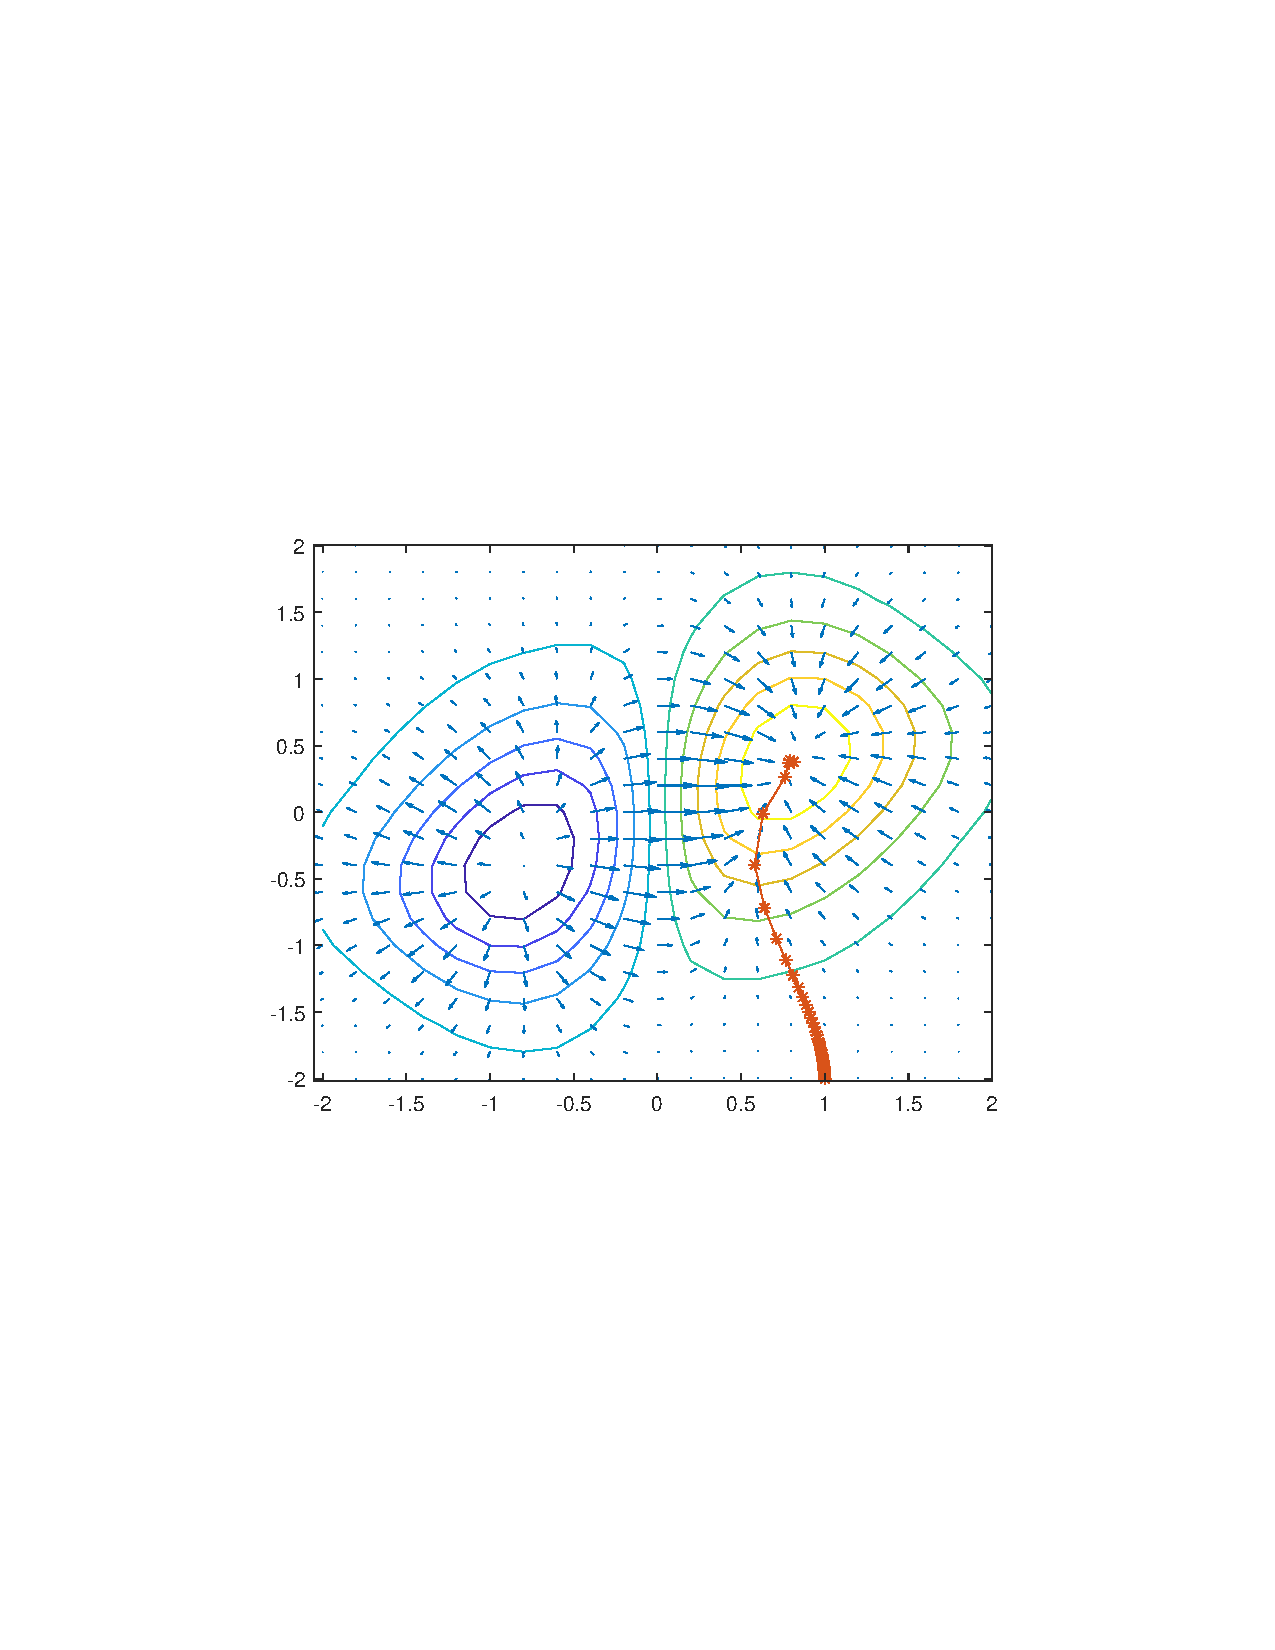
\includegraphics[width=0.49\textwidth, trim = 5cm 9cm 4cm 9cm]{grad_ascent_quiver}}
	{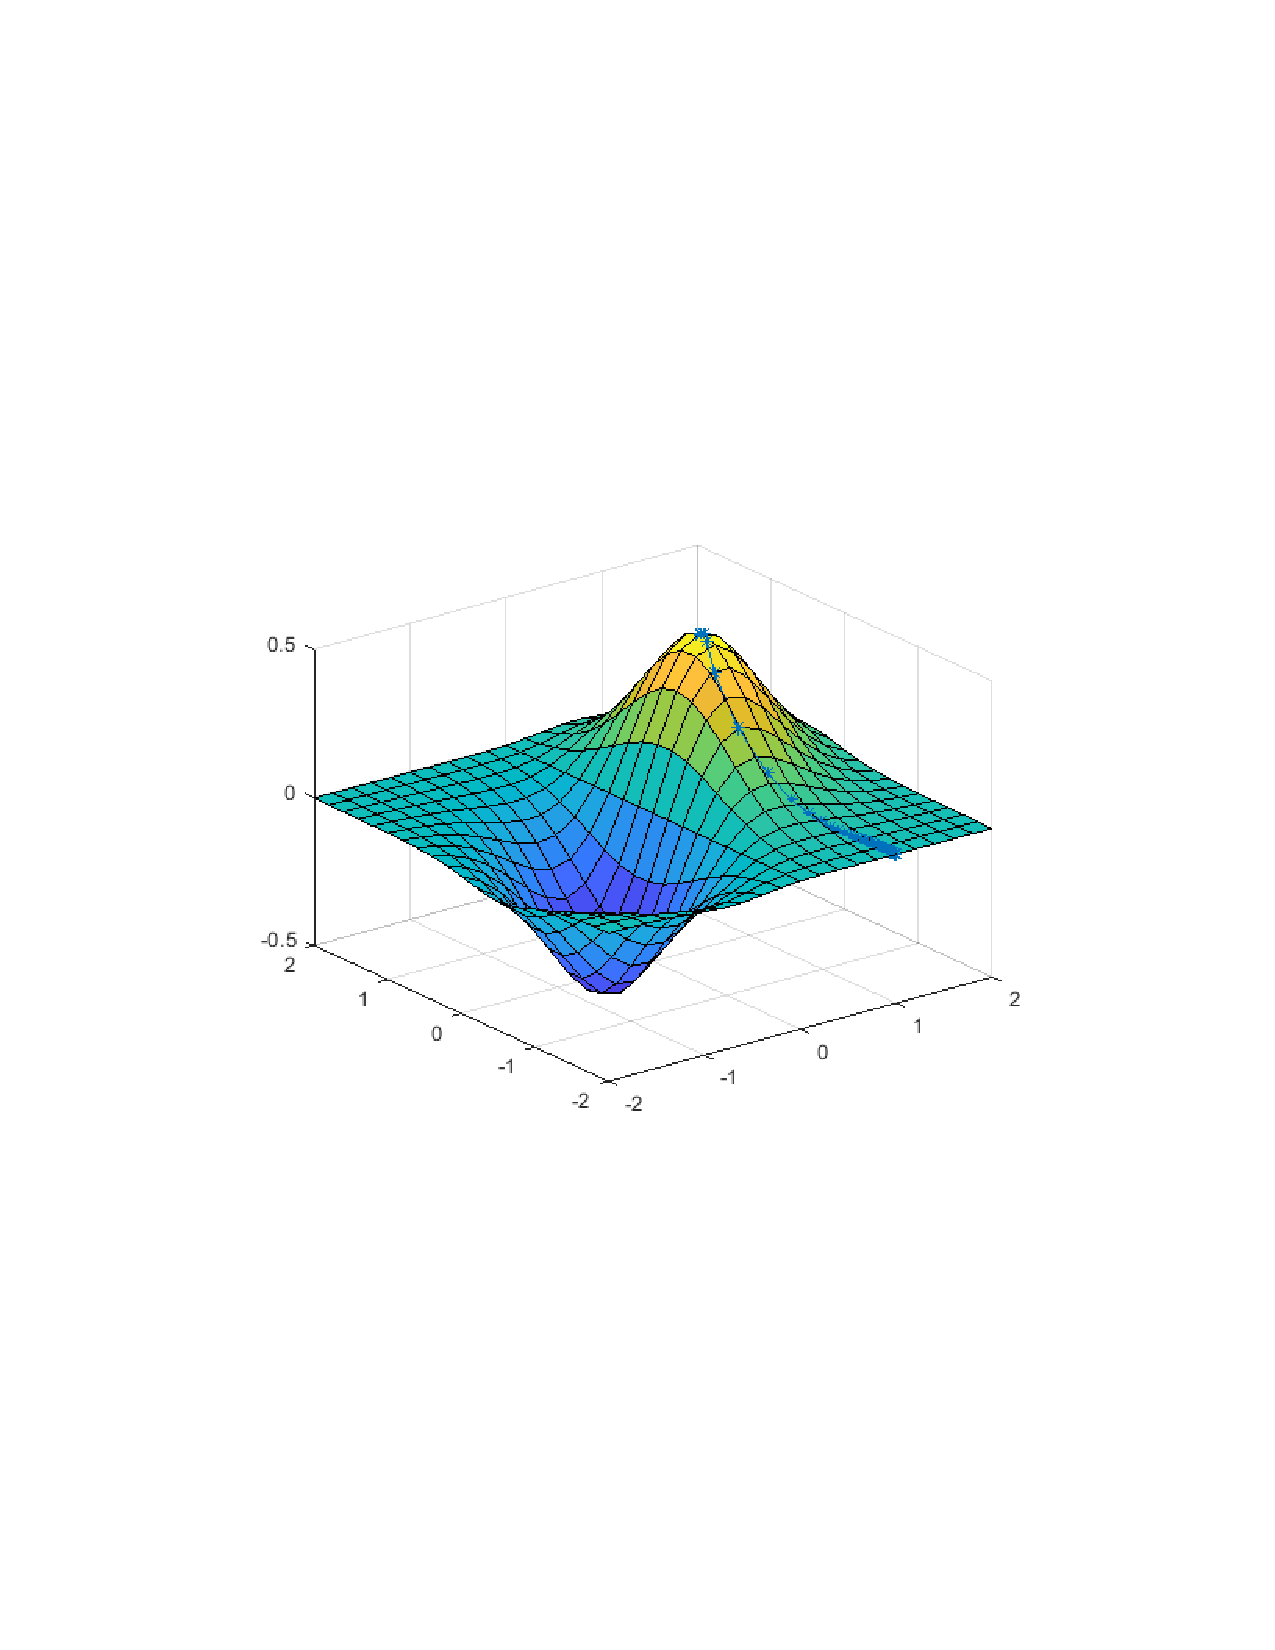
\includegraphics[width=0.49\textwidth, trim = 4cm 9cm 4cm 9cm]{grad_ascent_surf}}
	\caption{Gradient ascent on $f(x_1,x_2) = x_1e^{-x_1^2-x_.^2+\sin(x_1x_2)}$.}
	\label{fig:gradientascent}
\end{figure}
Since the gradient vector field may change from point to point, we can only ``follow" it numerically in finite
steps.  That is, starting from an initial guess $\mathbf{x}_0$,
we generate a sequence of points by the formula
$$
    \mathbf{x}_{n+1} = \mathbf{x}_n + \epsilon \nabla f(\mathbf{x}_n).
$$
The hope then is that
$$
      \mathbf{x}_n  \rightarrow \mathbf{x}^*.
$$
The number $\epsilon$ is often called the ``learning rate". It should not be too small or too large.
 If it is too small the
algorithm will be slow. If it is too large, the steps might skip over a critical point.
There is ongoing research about how to choose it optimally.

Notice the similarities between this method and the Newton's method for nonlinear systems in Lecture~\ref{lec:multnewton}.
In both cases we have a function of a vector and generate a sequence of vectors $\mathbf{x}_0,\mathbf{x}_1,\dots$.

%%%%%%%%%%%%%%%%%%%%%%%%

\subsection*{Exercises}
\begin{list}
  {\arabic{chapter}.\arabic{exercise}}{\usecounter{exercise}}

\item \label{exr:plotquiver}
Find by hand the gradient of the function $f(x_1,x_2) = \sin(x_1) \ e^{-x_1^2 - x_2^2}$. 
   Plot it on the rectangle
  $-3 \le x_1 \le 3$, $-2 \le x_2 \le 2$ using \verb&meshgrid& and \verb&quiver&. 
  On the same figure, add the contour plot of~$f$.


\item  Write a well-commented {\bf script} program that uses the gradient descent method to find a minimum point for the function $f(x_1,x_2) = \sin(x_1) \ e^{-x_1^2 - x_2^2}$, starting from $\mathbf{x}_0 = [-1;-2]$. 
Compare with the plot in exercise \ref{sec:maxmingrad}.\ref{exr:plotquiver} to check that it worked.
(Hint: Review the program \verb*|mymultnewton| in Lecture~\ref{lec:multnewton} for examples of making functions of vectors.)

\end{list}




%%%%%%%%%%%%%%%%%%%%%%%%%%%%%%%%%%%%%%%%%%%%%%%%%%%%%%%%%%%

\chapter{Double Integrals for Rectangles}


%%%%%%%%%%%%%%%%%%%%%%%%%%%%%

\subsection*{The center point method}

Suppose that we need to find the integral of a function,
$f(x,y)$, on a rectangle
$$
    R = \{(x,y): a\le x \le b, c \le y \le d\}.
$$
Calculus tells us to do this by an iterated integral
$$
 I = \iint_R f \, dA = \int_a^b \int_c^d f(x,y) \, dy dx
                   = \int_c^d \int_a^b f(x,y) \, dx dy.
$$
For instance, if $R$ is the rectangle $0 \le x \le 2$, $1 \le y \le 3$, then
\begin{equation*}
\begin{split}
  \iint_R x^2 y \, dA &= \int_0^2 \left(\int_1^3 x^2 y \, dy \right) \, dx \\
           &= \int_0^2  x^2 \left(\left. \frac{y^2}{2} \right|_1^3 \right) \, dx \\
           &= \int_0^2 x^2  \left( \frac{9}{2} - \frac{1}{2} \right) \, dx \\
           &= 4 \int_0^2 x^2 \, dx\\
           &= 4 \cdot \frac{8}{3} = \frac{32}{3} = 10.66... .
\end{split}
\end{equation*}

Calculus also tells us that the integral
is the limit of the  Riemann sums of the function as the size
of the subrectangles goes to zero. This means that the
Riemann sums are approximations of the integral, which is
precisely what we need for numerical methods.

For a rectangle $R$, we begin by subdividing into smaller
subrectangles $\{R_{ij}\}$, in a systematic way. We will divide
$[a,b]$ into $m$ subintervals and $[c,d]$ into $n$ subintervals.
Then $R_{ij}$ will be the ``intersection'' of the $i$-th subinterval
in $[a,b]$ with the $j$-th subinterval of $[c,d]$. In this way
the entire rectangle is subdivided into $mn$ subrectangles, numbered
as in Figure~\ref{rects}.
\begin{figure}
\begin{center}
\setlength{\unitlength}{0.9 mm}
\begin{picture}(83,53)(-3,-3)
	\put(0,0){\line(1,0){80}}
	\put(0,10){\line(1,0){80}}
	\put(0,20){\line(1,0){80}}
	\put(0,30){\line(1,0){80}}
	\put(0,40){\line(1,0){80}}
	\put(0,50){\line(1,0){80}}
	\put(0,0){\line(0,1){50}}
	\put(20,0){\line(0,1){50}}
	\put(40,0){\line(0,1){50}}
	\put(60,0){\line(0,1){50}}
	\put(80,0){\line(0,1){50}}
%
	\put(0,-3){\mbox{$a$}}
	\put(79,-4){\mbox{$b$}}
	\put(-3,0){\mbox{$c$}}
	\put(-3,49){\mbox{$d$}}
%
	\put(5,5){\mbox{$R_{11}$}}
	\put(25,5){\mbox{$R_{21}$}}
	\put(45,5){\mbox{$R_{31}$}}
	\put(65,5){\mbox{$R_{41}$}}
	\put(5,15){\mbox{$R_{12}$}}
	\put(5,25){\mbox{$R_{13}$}}
	\put(5,35){\mbox{$R_{14}$}}
	\put(5,45){\mbox{$R_{15}$}}
	\put(25,15){\mbox{$R_{22}$}}
	\put(25,25){\mbox{$R_{23}$}}
	\put(25,35){\mbox{$R_{24}$}}
	\put(25,45){\mbox{$R_{25}$}}
	\put(45,15){\mbox{$R_{32}$}}
	\put(45,25){\mbox{$R_{33}$}}
	\put(45,35){\mbox{$R_{34}$}}
	\put(45,45){\mbox{$R_{35}$}}
	\put(65,15){\mbox{$R_{42}$}}
	\put(65,25){\mbox{$R_{43}$}}
	\put(65,35){\mbox{$R_{44}$}}
	\put(65,45){\mbox{$R_{45}$}}
\end{picture}
\end{center}
\caption{Subdivision of the rectangle $R = [a,b] \times [c,d]$ into
         subrectangles $R_{ij}$. Note that the arrangement in the $x$-$y$ plane is completely different from the convention in a matrix.}
\label{rects}
\end{figure}

A Riemann sum using this subdivision would have the form 
$$ S =
\sum_{i,j=1,1}^{m,n} f(x^*_{ij}) A_{ij} = \sum_{j=1}^n
\left(\sum_{i=1}^m f(x^*_{ij}) A_{ij}\right)\,, 
$$ where $A_{ij} =
\Delta x_i \Delta y_j$ is the area of $R_{ij}$, and $x^*_{ij}$ is a
point in $R_{ij}$. The theory of integrals tells us that if $f$ is
continuous, then this sum will converge to the same number, no matter
how we choose $x^*_{ij}$. For instance, we could choose $x^*_{ij}$ to
be the point in the lower left corner of $R_{ij}$ and the sum would
still converge as the size of the subrectangles goes to zero. However,
in practice we wish to choose $x^*_{ij}$ in such a way to make $S$ as
accurate as possible even when the subrectangles are not very
small. The obvious choice for the best point in $R_{ij}$ would be the
center point. The center point is most likely of all points to have a
value of $f$ close to the average value of $f$. If we denote the
center points by $c_{ij}$, then the sum becomes
\[ C_{mn} =
\sum_{i,j=1,1}^{m,n} f(c_{ij}) A_{ij}.
\]
Here
\[
 c_{ij} = \left(
\frac{x_{i-1} + x_i}{2}, \frac{y_{i-1} + y_i}{2} \right).
\]
 Note
that if the subdivision is evenly spaced then $\Delta x \equiv
(b-a)/m$ and $\Delta y \equiv (d-c)/n$, and so in that case
\[
 C_{mn}
= \frac{(b-a)(d-c)}{mn} \sum_{i,j=1,1}^{m,n} f(c_{ij}).
\]


%%%%%%%%%%%%%%%%%%

\subsection*{The four corners method}

Another good idea would be to take the value of $f$ not only at one
point, but as the average of the values at several points. An obvious
choice would be to evaluate $f$ at all four corners of each $R_{ij}$
then average those. If we note that the lower left corner is
$(x_i,y_j)$, the upper left is $(x_i,y_{j+1})$,
the lower right is $(x_{i+1},y_i)$ and the upper right is
$(x_{i+1},y_{i+1})$, then the corresponding sum will be
$$
   F_{mn} =   \sum_{i,j=1,1}^{m,n} \frac{1}{4}
            \left( f(x_i,y_j) +
                   f(x_i,y_{j+1}) +
                   f(x_{i+1},y_i) +
                   f(x_{i+1},y_{j+1}) \right)    A_{ij},
$$
which we will call the {\em four-corners} method.
If the subrectangles are evenly spaced, then we can simplify this
expression. Notice that $f(x_i,y_j)$ gets counted multiple
times depending on where $(x_i,y_j)$ is located. For instance
if $(x_i,y_j)$ is in the interior of $R$ then it is the corner
of $4$ subrectangles. Thus the sum becomes
$$
F_{mn} = \frac{A}{4} \left( \sum_{\text{corners}} f(x_i,y_j)
                   + 2 \sum_{\text{edges}} f(x_i,y_j)
                   + 4 \sum_{\text{interior}} f(x_i,y_j)
                         \right),
$$
where $A = \Delta x \, \Delta y$ is the area of the subrectangles.
We can think of this as a weighted average of the values of $f$ at
the grid points $(x_i,y_j)$. The weights used are represented in
the matrix
\begin{equation}\label{dbltrapmatrix}
W = \left( \begin{array}{cccccccc}
           1 & 2 & 2 & 2 & \cdots & 2 & 2 & 1 \\
           2 & 4 & 4 & 4 & \cdots & 4 & 4 & 2 \\
           2 & 4 & 4 & 4 & \cdots & 4 & 4 & 2 \\
        \vdots & \vdots & \vdots & \vdots & \cdots & \vdots & \vdots & \vdots \\
           2 & 4 & 4 & 4 & \cdots & 4 & 4 & 2 \\
           1 & 2 & 2 & 2 & \cdots & 2 & 2 & 1 \\
           \end{array}
    \right).
\end{equation}
We could implement the four-corner method by forming a matrix $(f_{ij})$
of $f$ values at the grid points, then doing entry-wise multiplication
of the matrix with the weight matrix. Then the integral would be
obtained by summing all the entries of the resulting matrix and
multiplying that by $A/4$. The formula would be
$$
     F_{mn} = \frac{(b-a)(d-c)}{4mn} \sum_{i,j = 1,1}^{m+1,n+1}
                       W_{ij} f(x_i,y_j).
$$
Notice that the four-corners method coincides with applying the trapezoid
rule in each direction. Thus it is in fact a {\em double trapezoid}\/ rule.


%%%%%%%%%%%%%%%%%%%%%%%%%%%%

\subsection*{The double Simpson method}

The next improvement one might make would be to take an average of
the center point sum $C_{mn}$ and the four corners sum $F_{mn}$.
However, a more standard way to obtain a more accurate method
is the Simpson double integral. It is obtained by applying Simpson's
rule for single integrals to the iterated double integral.
The resulting method requires that both $m$ and $n$ be even numbers
and the grid be evenly spaced. If this is the case we sum up the
values $f(x_i,y_j)$ with weights represented in the matrix
\begin{equation}\label{dblsimpmatrix}
W = \left( \begin{array}{cccccccc}
           1 & 4 & 2 & 4 & \cdots & 2 & 4 & 1 \\
           4 & 16 & 8 & 16 & \cdots & 8 & 16 & 4 \\
           2 & 8 & 4 & 8 & \cdots & 4 & 8 & 2 \\
           4 & 16 & 8 & 16 & \cdots & 8 & 16 & 4 \\
        \vdots & \vdots & \vdots & \vdots & \cdots & \vdots & \vdots & \vdots \\
           2 & 8 & 4 & 8 & \cdots & 4 & 8 & 2 \\
           4 & 16 & 8 & 16 & \cdots & 8 & 16 & 4 \\
           1 & 4 & 2 & 4 & \cdots & 2 & 4 & 1 \\
           \end{array}
    \right).
\end{equation}
The sum of the weighted values is multiplied by $A/9$ and the formula is
$$
     S_{mn} = \frac{(b-a)(d-c)}{9mn} \sum_{i,j = 1,1}^{m+1,n+1}
                       W_{ij} f(x_i,y_j).
$$


\textsc{Matlab} has a built in command for double integrals on
rectangles: \verb&integral2(f,a,b,c,d)&. Here is an example:
\begin{lstlisting}[frame=none,numbers=left]
f = @(x,y) sin(x.*y)./sqrt(x+y)
I = integral2(f,0.5,1,0.5,2)
\end{lstlisting}
Note that here, as usual, operations are component-wise.

Below is a \textsc{Matlab} function which will produce the
matrix of weights needed for Simpson's rule for double integrals.
It uses the function \verb&mysimpweights& from Lecture~22.


\lstinputlisting{../programs/mydblsimpweights.m}


%%%%%%%%%%%%%%%%


\subsection*{Exercises}
\begin{list}
{\arabic{chapter}.\arabic{exercise}}{\usecounter{exercise}}

\item Download the program \programlink{mylowerleft.m} and test it.
  Find and fix the bug in it.
  Modify it to make a new program \verb&mycenter& that does the center
  point method. Implement the change by changing the ``meshgrid'' to
  put the grid points at the centers of the subrectangles. Look at the
  mesh plot produced to make sure the program is putting the grid
  where you want it. Use both programs to approximate the integral
  $$
  \int_0^2 \int_1^5 \sqrt{xy} \, dy \, dx,
  $$
  using $(m,n) = (10,18)$.  Evaluate this integral exactly (by hand) and compare
  the accuracy of the two programs.

\item Write a well-commented \textsc{Matlab} {\bf function} program
  \verb&mydblsimp& that computes the Simpson's rule approximation. Let
  it call the program \verb&mydblsimpweights& (above) to make the weight
  matrix, $w$ (\ref{dblsimpmatrix}). Check the program on
  the integral in the previous problem using  $(m,n) = (10,18)$ and $(m,n) = (100,100)$.

\item Using \verb&mysimpweights& and \verb&mydblsimpweights& as models
  make well-commented \textsc{Matlab} {\bf function} programs
  \verb&mytrapweights& and \verb&mydbltrapweights& that will produce
  the weights for the trapezoid rule and the weight matrix for the
  four corners (double trapezoid) method (\ref{dbltrapmatrix}). 
  Use it to approximate the integral in the previous problem usings  $(m,n) = (5,6)$ and $(m,n) = (100,100)$.
  Turn in the programs, the weights for a $5\times 6$ grid, and the results of your tests on the integral.

\end{list}

%%%%%%%%%%%%%%%%%%%%%%%%%%%%%%%%%%%%%%%%%%%%%%%%%%%%%%%%%%%%%%%%%

\chapter{Double Integrals for Non-rectangles}


In the previous lecture we considered only integrals over
rectangular regions. In practice, regions of interest are
rarely rectangles and so in this lecture we consider two
strategies for evaluating integrals over other regions.

Calculus tells us that if the region can be described by simple functions,
then we might be able to use iterated integrals. For instance, suppose that
$R$ is the region inside of a circle of radius $2$. Since the boundary of that
circle is given by $x^2 + y^2 = 2^2$,  we could express the
integral of $f(x,y)$ on this region by:
$$
  \int_{-2}^2 \int_{-\sqrt{4-x^2}}^{ \sqrt{4-x^2}} f(x,y) \, dy dx.
$$
Of course this integral may be complicated, even if $f(x,y)$ is simple.
If $f(x,y) = x^2 y^2$, then
\begin{equation*}
\begin{split}
  \int_{-2}^2 \int_{-\sqrt{4-x^2}}^{ \sqrt{4-x^2}} x^2 y^2 \, dy dx 
          &=  \int_{-2}^2 \left. x^2 \frac{y^3}{3} \right|_{-\sqrt{4-x^2}}^{ \sqrt{4-x^2}} \,  dx  \\
          &=  \frac{2}{3} \int_{-2}^2  x^2 (4 - x^2)^\frac{3}{2}  \, dx.     
\end{split}
\end{equation*}
At this point we would need to do a trig substitution to find the value of the integral.

%%%%%%%%%%%%%%%%%%%%%%%%%%%%%

\subsection*{Redefining the function}

One strategy is to redefine the function so that it is zero
outside the region of interest, then integrate over a rectangle
that includes the region.

For example, suppose we need to approximate the value
of
$$
    I = \iint_T \sin^3 (xy) \, dx \, dy
$$
where $T$ is the triangle with corners at $(0,0)$, $(1,0)$ and $(0,2)$.
Then we could let $R$ be the rectangle $[0,1] \times [0,2]$ which
contains the triangle $T$. Notice that the hypotenuse of the triangle
has the equation $2x + y = 2$. Then make $f(x) = \sin^3 (xy)$ if $2x +y \le 2$
and $f(x) = 0$ if $2x+y > 2$.
In \textsc{Matlab} we can make this function with the command
\begin{lstlisting}[frame=none,numbers=left]
f = @(x,y) sin(x.*y).^3.*(2*x + y <= 2)
\end{lstlisting}
In this command \verb&<=& is a {\em logical}\/ command. The term
in parentheses is then a {\em logical statement}\/ and is given the
value 1 if the statement is true and 0 if it is false.
We can then integrate the modified \verb&f& on $[0,1] \times [0,2]$
using the command
\begin{lstlisting}[frame=none,numbers=left]
I = integral2(f,0,1,0,2)
\end{lstlisting}

As another example, suppose we need to integrate the function $f(x,y) = 10+(x-1)(y-2)$
inside the circle of radius 2 centered at $(1,2)$. The equation for
this circle is $(x-1)^2 + (y-2)^2 = 4$. Note that the inside of the
circle is $(x-1)^2 + (y-2)^2 \le 4$ and that the circle is contained
in the rectangle $[-1,3] \times [0,4]$. Thus  we can create
the right function, plot it, and integrate it by
\begin{lstlisting}[frame=none,numbers=left]
f = @(x,y) (10+(x-1).*(y-2)).*((x-1).^2 + (y-2).^2 <= 4)
[X Y] = meshgrid(-4:0.01:4,-3:0.01:5);
Z = f(X,Y);
mesh(X,Y,Z)
I = integral2(f,-1,3,0,4)
\end{lstlisting}

%%%%%%%%%%%%%%%%%%%%%

\subsection*{Integration Based on Triangles}

The second approach to integrating over non-rectangular regions
is based on subdividing the region into triangles. Such a subdivision
is called a {\em triangulation}. On regions
where the boundary consists of line segments, this can be done exactly.
Even on regions where the boundary contains curves, this can be done
approximately. This is a very important idea for several reasons, the
most important of which is that the finite elements method is based on it.
Another reason this is important is that often the values of
$f$ are not given by a formula, but from data.
For example, suppose you are surveying on a construction site
and you want to know how much fill will be needed to bring the
level up to the plan. You would proceed by taking elevations
at numerous points across the site. However, if the site is
irregularly shaped or if there are obstacles on the site, then
you cannot make these measurements on an exact rectangular grid.
In this case, you can use triangles by connecting your points
with triangles. Many software packages will even choose the
triangles for you (\textsc{Matlab} will do it using the command
\verb&delaunay&).

The basic idea of integrals based on triangles is exactly the same
as that for rectangles; the integral is approximated by a sum
where each term is a value times an area
$$
   I \approx \sum_{i=1}^n f(x^*_i) A_i
\,,
$$
where $n$ is the number of triangles, $A_i$ is the area of the triangle
and $x^*$ a point in the triangle. However, rather than considering
the value of $f$ at just one point people often consider an average
of values at several points. The most convenient of these is of course
the corner points. We can represent this sum by
$$
   T_n = \sum_{i=1}^n \bar{f}_i A_i
\,,
$$
where $\bar{f}$ is the average of $f$ at the corners.

If the triangle has vertices $(x_1,y_1)$, $(x_2,y_2)$
and $(x_3,y_3)$,  the formula for area is
\begin{equation}\label{triarea}
A =
\frac{1}{2}\left|
\text{det}\left(
\begin{array}{ccc}
x_1	&x_2	&x_3\\
y_1	&y_2	&y_3\\
1	&1	&1\\
\end{array}
\right)
\right|
% likely wrong, may assume certain differences >0
%A = \frac{1}{2}(x_3 - x_1)(y_2 - y_1) - \frac{1}{2} (y_3 - y_1)(x_2 - x_1)
.
\end{equation}
The function \programlink{mythreecorners.m} below implements this method.
\lstinputlisting{../programs/mythreecorners.m}

Another idea would be to use the center point (centroid) of
each triangle. If the triangle has vertices $(x_1,y_1)$, $(x_2,y_2)$
and $(x_3,y_3)$, then the centroid is given by the simple
formulas
\begin{equation}\label{tricenter}
\bar{x} = \frac{x_1 + x_2 + x_3}{3}
\quad\text{and}\quad
\bar{y} = \frac{y_1 + y_2 + y_3}{3}.
\end{equation}


%%%%%%%%%%%%

\subsection*{Exercises}
\begin{list}
{\arabic{chapter}.\arabic{exercise}}{\usecounter{exercise}}


\item  
   \begin{enumerate}
      \item[a.] Download the program \programlink{mywasher.m}.
      Plot $f(x,y) = \frac{x+y}{x^2+y^2}$ on the region produced  by \programlink{mywasher.m} and 
      use the program \programlink{mythreecorners.m} to calculate the integral of $f$ on the washer.
      Is this accurate? How do you know?
      \item[b.] Download the program \programlink{mywedge.m}.
      Plot $g(x,y) = \sin(x) + \sqrt{y}$ on the region produced  by \programlink{mywedge.m}
      use \programlink{mythreecorners.m} to calculate the integral of $g$ on this wedge.
   \end{enumerate}

\item
  Modify the program \programlink{mythreecorners.m}
  to a new program
\verb&mycenters.m& that does the centerpoint method for triangles. Run
the program on the region produced by \programlink{mywasher.m} with the
function $f(x,y) = \frac{x+y}{x^2+y^2}$ and on the region produced by
\programlink{mywedge.m} with the function $g(x,y) = \sin(x) + \sqrt{y}$.

\end{list}

%
%
%%%%%%%%%%%%%%%%%%%%%%%%%%%%%%%%%%%%%%%%%%%%%%%%%%%%%%%%%%%%%%%%
%
%
%
%\chapter{Gaussian Quadrature*}
%
%
%%%%%%%%%%%%%%%%%%%%%%%%%%%%%%
%
%
%\subsection*{Exercises}
%\begin{list}
%{\arabic{chapter}.\arabic{exercise}}{\usecounter{exercise}}
%
%\item
%
%\vspace*{.2in}
%
%\item
%
%\end{list}
%

%%%%%%%%%%%%%%%%%%%%%%%%%%%%%%%%%%%%%%%%%%%%%%%%%%%%%%

\chapter{Numerical Differentiation}


%%%%%%%%%%%%%%%%%%%%%%%%%%%%%

\subsection*{Approximating derivatives from data}


Suppose that a variable $y$ depends on another variable $x$,
i.e.~$y = f(x)$, but we only know the values of $f$
at a finite set of points, e.g., as data from an experiment
or a simulation:
$$
 (x_1,y_1), (x_2,y_2), \ldots, (x_n,y_n).
$$
Suppose then that we need information about the derivative of $f(x)$.
One obvious idea would be to approximate $f'(x_i)$ by the {\bf Forward
  Difference}
$$
f'(x_i) = y'_i \approx \frac{y_{i+1} - y_i}{x_{i+1}-x_i}.
$$
This formula follows directly from the definition of the derivative in
Calculus.  An alternative would be to use a {\bf Backward Difference}
$$
f'(x_i) \approx \frac{y_i - y_{i-1}}{x_i-x_{i-1}}.
$$

Since the errors for the  forward difference and backward difference tend
to have opposite signs, it would seem likely that averaging the two
methods would give a better result than either alone. If the points are
evenly spaced, i.e.\ $x_{i+1}-x_i = x_i-x_{i-1} = h$, then averaging the
forward and backward differences leads to a symmetric expression called
the {\bf Central Difference}
$$
f'(x_i) = y'_i \approx \frac{y_{i+1} - y_{i-1}}{2h}.
$$
See Figure~\ref{fig:FBCdifferences} for an illustration of these three differences.

\begin{figure}
\centerline{
\includegraphics[width=0.7\textwidth]{differences}}
\caption{The three difference approximations of $y'_i$.}
\label{fig:FBCdifferences}
\end{figure}



%%%%%%%%%%%%%%%%%%%%%%%%%%%%%%


\subsection*{An example}
The following code plots the function $y = \sin(x) + .5\sin(1.5x)$, its derivative, and the central difference approximation to the derivative.

\begin{lstlisting}[frame=none,numbers=left]
x = linspace(0,2*pi,51);
h = x(2)-x(1);
mid = (x(1:end-1)+x(2:end))/2;
y = sin(x) + .5*sin(1.5*x);
dy1 = (y(2:end)-y(1:end-1))/h;
dy2 = cos(x) + .75*cos(1.5*x);
plot(x,y,'k',mid,dy1,'b*',x,dy2,'r')
\end{lstlisting}

%%%%%%%%%%%%%%%%%%%%%%%%%%%%%

\subsection*{Errors of approximation}

We can use Taylor polynomials to derive the accuracy of the forward,
backward, and central difference formulas. For example the usual form
of the Taylor polynomial with remainder (sometimes called Taylor's
Theorem) is
\[ 
f(x+h) = f(x) + h f'(x) + \frac{h^2}{2} f''(c)\,, 
\]
where $c$ is some (unknown) number between $x$ and $x+h$. Letting $x =
x_i$, $x+h = x_{i+1}$ and solving for $f'(x_i)$ leads to
$$ f'(x_i) =
\frac{f(x_{i+1})-f(x_i)}{h} - \frac{h}{2} f''(c).  
$$ 
Notice that the
quotient in this equation is exactly the forward difference formula.
Thus the error of the forward difference is $- (h/2) f''(c)$ which
means it is $O(h)$.  Replacing $h$ in the above calculation by $-h$
gives the error for the backward difference formula; it is also
$O(h)$. For the central difference, the error can be found from the
third degree Taylor polynomials with remainder
\begin{align*}
f(x_{i+1}) &= f(x_i + h)
= f(x_i) + hf'(x_i)+ \frac{h^2}{2} f''(x_i) + \frac{h^3}{3!} f'''(c_1)
\quad\text{and}\\
f(x_{i-1}) &= f(x_i - h)
= f(x_i) - hf'(x_i)+ \frac{h^2}{2} f''(x_i) - \frac{h^3}{3!} f'''(c_2)
\,,
\end{align*}
where $x_i \le c_1 \le x_{i+1}$ and $x_{i-1} \le c_2 \le x_i$.
Subtracting these two equations and solving for $f'(x_i)$ leads to
$$
    f'(x_i) = \frac{f(x_{i+1})-f(x_{i-1})}{2h}
    - \frac{h^2}{3!} \frac{f'''(c_1) + f'''(c_2)}{2}.
$$
This shows that the error for the central difference formula is $O(h^2)$.
Thus, central differences are significantly better and so:
{\bf It is best to use central differences whenever possible.}

There are also central difference formulas for higher order
derivatives. These all have error of order $O(h^2)$:
\begin{align*}
f''(x_i) &=
y''_i \approx \frac{y_{i+1} - 2 y_i + y_{i-1}}{h^2},\\
f'''(x_i) &=
y'''_i \approx \frac{1}{2 h^3} \left[y_{i+2} - 2y_{i+1} + 2y_{i-1} -
y_{i-2} \right] ,\quad\text{and}\\
f^{(4)}(x_i) &= y^{(4)}_i \approx \frac{1}{h^4}
\left[y_{i+2} - 4y_{i+1} + 6y_i - 4y_{i-1} + y_{i-2} \right]
.
\end{align*}

%%%%%%%%%%%%%%%%%%%%%%%%%%%%%

\subsection*{Partial Derivatives}

Suppose $u = u(x,y)$ is a function of two variables that we
only know at grid points $(x_i,y_j)$. We will use the notation
$$
      u_{i,j} = u(x_i,y_j)
$$
frequently throughout the rest of the lectures.
We can suppose that the grid points are evenly spaced, with
an increment of $h$ in the $x$ direction and $k$ in the $y$ direction.
The central difference formulas for the partial derivatives
would be
\begin{align*}
u_x(x_i,y_j) &\approx \frac{1}{2h}
                      \left( u_{i+1,j} - u_{i-1,j} \right)
\quad\text{and}\\
u_y(x_i,y_j) &\approx \frac{1}{2k}
                      \left( u_{i,j+1} - u_{i,j-1} \right).
\end{align*}
The second partial derivatives are
\begin{align*}
u_{xx}(x_i,y_j) &\approx \frac{1}{h^2}
                    \left( u_{i+1,j} -2u_{i,j} + u_{i-1,j} \right)
\quad\text{and}\\
u_{yy}(x_i,y_j) &\approx \frac{1}{k^2}
                    \left( u_{i,j+1} -2u_{i,j} + u_{i,j-1} \right) ,
\end{align*}
and the mixed partial derivative is
$$
    u_{xy}(x_i,y_j) \approx \frac{1}{4hk}
  \left( u_{i+1,j+1} - u_{i+1,j-1} - u_{i-1,j+1} + u_{i-1,j-1} \right) .
$$

{\bf Caution:} Notice that we have indexed $u_{ij}$ so that as a matrix
each row represents the values of $u$ at a certain $x_i$ and each column
contains values at $y_j$. The arrangement in the matrix does not
coincide with the usual orientation of the $xy$-plane.

Let's consider an example. Let the values of $u$ at $(x_i,y_j)$ be
recorded in the matrix
\begin{equation}\label{umatrix}
(u_{ij}) =
 \left( \begin{array}{ccccc}
        5.1 & 6.5 & 7.5 & 8.1 & 8.4 \\
        5.5 & 6.8 & 7.8 & 8.3 & 8.9 \\
        5.5 & 6.9 & 9.0 & 8.4 & 9.1 \\
        5.4 & 9.6 & 9.1 & 8.6 & 9.4
           \end{array} \right)
\end{equation}
Assume the indices begin at 1, $i$ is the index for rows and $j$ the index for columns. Suppose that $h = .5$ and $k = .2$. Then $u_y(x_2,y_4)$ would be
approximated by the central difference
$$
u_y(x_2,y_4) \approx \frac{u_{2,5} - u_{2,3}}{2k}
               \approx \frac{8.9 - 7.8}{2 \cdot 0.2} = 2.75.
$$
The partial derivative $u_{xy}(x_2,y_4)$ is approximated by
$$
u_{xy}(x_2,y_4) \approx \frac{u_{3,5} - u_{3,3} - u_{1,5} + u_{1,3}}{4hk}
               \approx \frac{9.1 - 9.0 - 8.4 + 7.5}{4\cdot .5 \cdot .2}
                 = -2.
$$


%%%%%%%%%%%%%%%%%%%%%%%%%%%%%

\subsection*{Exercises}


\begin{list}
{\arabic{chapter}.\arabic{exercise}}{\usecounter{exercise}}

\item Suppose you are given the data in the following table.\\
\begin{tabular}{c|ccccc}
x & 0 & 5 & 10 & 15 & 20 \\ \hline
y & 0 & 19 & 26 & 29 & 31
\end{tabular}\\
a. Give the forward, backward and central difference approximations of $f'(5)$.\\
b. Give the central difference approximations for $f''(10)$, $f'''(10)$ and
   $f^{(4)}(10)$.
   
\item Suppose the position of a runner was recorded every half second and the results
are given in the following table. Units of distance are meters.\\
\begin{tabular}{c|ccccccccccccc}
t & 0 & .5   & 1.0 & 1.5 & 2.0 & 2.5 & 3.0 & 3.5 & 4.0 & 4.5 & 5.0 & 5.5 & 6.0 \\ \hline
y & 0 & .25 & 1   &   3  & 6    & 10  & 15  & 21  & 27  & 33  &  39  & 45  & 51
 \end{tabular}\\
 Using central differences everywhere possible, and a forward or backward difference where
a central difference is not possible, calculate and plot the velocity and the acceleration of the runner
as a function of time for t=0 to 6. You may do the calculations by hand or by \textsc{Matlab}.  
Turn in your plots and calculations.

\item Suppose values of $u(x,y)$ at points $(x_i,y_j)$ are given in the
matrix (\ref{umatrix}). Suppose that $h = .1$ and $k = .3$.
Approximate the following derivatives by central differences:\\
a. $u_x(x_3,y_4)$\\
b. $u_{xx}(x_2,y_2)$\\
c. $u_{yy}(x_3,y_4)$\\
d. $u_{xy}(x_3,y_3)$


\end{list}




%%%%%%%%%%%%%%%%%%%%%%%%%%%%%%%%%%%%%%%%%%%%%%%%%%%%%%%%%%%%%

\chapter{The Main Sources of Error}

%(not counting bugs)

%%%%%%%%%%%%

\subsection*{Truncation Error}

Truncation error is defined as the error caused directly by an
approximation method. For instance, all numerical integration methods
are approximations and so there is error, even if the calculations are
performed exactly. Numerical differentiation also has a truncation
error, as will the differential equations methods we will study in
Part IV, which are based on numerical differentiation formulas. There
are two ways to minimize truncation error: (1) use a higher order
method, and (2) use a finer grid so that points are closer
together. Unless the grid is very small, truncation errors are usually
much larger than roundoff errors. The obvious tradeoff is that a
smaller grid requires more calculations, which in turn produces more
roundoff errors and requires more running time.

%%%%%%%%%%%%%%%%%%%%%%%%%%

\subsection*{Roundoff Error}

Roundoff error always occurs when a finite number of digits are recorded
after an operation. Fortunately, this error is extremely small. The standard
measure of how small is called {\bf machine epsilon}. It is defined as the
smallest number that can be added to $1$ to produce another number on
the machine, i.e.~if a smaller number is added the result will be rounded
down to $1$. In IEEE standard double precision (used by \textsc{Matlab}
and most serious software), machine epsilon is $2^{-52}$ or about
$2.2 \times 10^{-16}$. A different, but equivalent, way of thinking about
this is that the machine records $52$ floating binary digits or about $15$
floating decimal digits. Thus there are never more than $15$ significant digits
in any calculation. This of course is more than adequate for any application.
However, there are ways in which this very small error
can cause problems.

You can test that machine epsilon is $2^{-52}$:
\begin{lstlisting}[frame=none,numbers=left]
format long
(1 + 2^(-52)) - 1
(1 + 2^(-53)) - 1
\end{lstlisting}
\textsc{Matlab} has a command that produces machine epsilon:
\begin{lstlisting}[frame=none,numbers=left]
eps
\end{lstlisting}
To see an unexpected occurence of round-off try
\begin{lstlisting}[frame=none,numbers=left]
(2^52+1) - 2^52
(2^53+1) - 2^53
\end{lstlisting}
Thus roundoff isn't always small! It is just small compared with the scale of
the numbers you are calculating.
A number of magnitude \(10^p\) will have roundoff of magnitude about \(10^p\cdot 10^{-16}=10^{p-16}\). 

%%%%%%%%%%%%%%%%%%%%%

\subsection*{Loss of Precision (also called Loss of Significance)}

Suppose we had some way
to compute \(\pi\)
that effectively did the calculation
\((e\cdot10^{9}+\pi)-e\cdot10^{9}\). Rounding everything to 16 digits, 
we are computing
\[
(2718281828.459045
+3.141592653589793)
-2718281828.459045\,.
\]
The addition is performed first and the result rounded to 16 digits, giving
\[
 2718281831.600637 %4
-2718281828.459045
\,.
\]
Although roundoff caused some error, it is about a factor of
\(10^{-16}\)
smaller than the numbers shown. In other words, all but perhaps the
last digit shown is correct.
Next the subtraction is performed, giving
\[
 00 00 00 00 03.141592
\,.
\]
The leading zeros are not significant, so we lost 9 significant digits
and have only 7 left.  This type of error, where common leading
significant digits cancel, is loss-of-precision (also called
loss-of-significance) error.
Computers will not display these leading zeros. Instead, the subtraction above yielded  
\[
3.141592025756836
\,.
\]
Although it is displayed with 16 digits, only the first 7 are correct.
%
Usually, if you add two numbers of magnitude \(10^p\) each with roundoff error \(10^{p-16}\), then the result is also of magnitude \(10^p\) and the relative error due to roundoff is \(10^{p-16}/10^p=10^{-16}\).
In this example, cancellation made the result of magnitude \(10^{p-q}\), so the relative error due to roundoff is \(10^{p-16}/10^{p-q}=10^{q-16}\), and so we lost $q=9$ digits of precision.

This type of {\em loss of
  precision}\/ can happen by accident, with catastrophic results, if
you are not careful. For example in $f'(x)\approx (f(x+h)-f(x))/h$ you
will lose precision when $h$ gets too small. Try
\begin{lstlisting}[frame=none,numbers=left]
format long
format compact
f = @(x) x^2
for i = 1:30
   h = 10^(-i)
   df = (f(1+h)-f(1))/h
   relerr = (2-df)/2
end
\end{lstlisting}
At first the relative error decreases since truncation error is reduced. Then
loss of precision takes over and the relative error increases to 1. This happens because when
$f(1)$ and $f(1+h)$ become close, the subtraction ``cancels" digits.


%%%%%%%%%%%%

\subsection*{Bad Conditioning}

We encountered bad conditioning in Part II, when we talked about
solving linear systems.  Bad conditioning means that the problem is
unstable in the sense that small input errors can produce large output
errors. This can be a problem in a couple of ways. First, the
measurements used to get the inputs cannot be completely
accurate. Second, the computations along the way have roundoff
errors. Errors in the computations near the beginning especially can be
magnified by a factor close to the condition number of the matrix.
Thus what was a very small problem with roundoff can become a very big
problem.

It turns out that matrix equations are not the only place where condition
numbers occur. In any problem one can define the condition number
as the maximum ratio of the relative errors in the output versus input, i.e.
$$      \textrm{condition \# of a problem}
          = \max \left( \frac{\text{Relative error of output}}
                             {\text{Relative error of inputs}} \right).
$$
An easy example is solving a simple equation
$$
     f(x) = 0.
$$
Suppose that $f'$ is close to zero at the solution $x^*$. Then a very
small change in $f$ (caused perhaps by an inaccurate measurement of
some of the coefficients in $f$) can cause a large change in $x^*$.
It can be shown that the condition number of this
problem is $1/f'(x^*)$.


\subsection*{Summary}

\begin{table}[hb]
\label{tab:errors}
\begin{tabular}{|c|c|c|}
\hline
\ Error type:  \ & \ Whose fault is it? \ & \ How to mitigate it? \ \\ \hline
\ Truncation \ & \ the method  \  & \ higher-order method or  finer grid \ \\
\ Round-off  \ &  \ the computer  \  & \ usually okay, higher precision arithmetic \ \\ 
\ Loss of Precision \ & \  the programmer \  & \ avoid cancellation of significant digits \  \\
\ Bad Conditioning \ &  \ the problem  \ &  \ check answers, redesign if possible \ \\
\hline
\end{tabular}
\caption{A summary of the main sources of error.}
\end{table}



%%%%%%%%%%%%%%%%
%\subsection*{Build Up}
%
%In addition to these sources of error, there is a another factor
%one must consider that effects the accuracy of calculations: build up.
%Build up can occur when one does multiple calculations
%in the same problem. Each computation may have only a small amount of
%roundoff, truncation or conditioning errors, but adding all the
%small errors up can result in a big error.

%For example, this is one of the trade-offs of using a smaller grid.
%A smaller grid has smaller truncation, but more calculations. At some
%point the advantage is out-weighted by the disadvantage.

%%%%%%%%%%%%

\newpage

\subsection*{Exercises}

\begin{list}
{\arabic{chapter}.\arabic{exercise}}{\usecounter{exercise}}

\item Identify the (main) source of error in each case and propose a
  way to reduce this error if possible.
  \begin{enumerate}
  \item[(a)] If we do $(\sqrt{3})^2$ we should get 3, but if we check
    \begin{lstlisting}[frame=none,numbers=left]
mythree = (sqrt(3))^2
mythree-3
    \end{lstlisting}
    we find the error is 
    \verb&ans = -4.4409e-16&.
  \item[(b)] Since it is a quarter of a circle of radius 2, we should
    have $\int_0^2 \sqrt{4-x^2}dx=\frac{1}{4}\pi2^2=\pi$. We try to
    use \verb&mytrap& from Lecture~\ref{sec:LRTrules} and do
    \begin{lstlisting}[frame=none,numbers=left]
x = 0:.2:2;
y = sqrt(4-x.^2);
mypi = mytrap(x,y)
mypi-pi
    \end{lstlisting}
    and find the error is \verb&ans = -0.0371&.
  \end{enumerate}

\item \footnote{From {\em Numerical Linear Algebra} by L.~Trefethen and D.~Bau, SIAM, 1997.}
%Do the worksheet ``Build-up of Roundoff Errors" from
The function $f(x)=(x-2)^9$ could be evaluated as written, or first
expanded as $f(x)=x^9-18x^8+\cdots$ and then evaluated.
To find the expanded version, type
\begin{lstlisting}[frame=none,numbers=left]
syms x
expand((x-2)^9)
clear
\end{lstlisting}
To evaluate it without expansion, type
\begin{lstlisting}[frame=none,numbers=left]
f1 = @(x) (x-2).^9
x = 1.92:.001:2.08;
y1 = f1(x);
plot(x,y1,'blue')
\end{lstlisting}
To do it with expansion, convert the symbolic expansion above to an anonymous
function \verb&f2& and then type
\begin{lstlisting}[frame=none,numbers=left]
y2 = f2(x);
hold on
plot(x,y2,'red')
\end{lstlisting}
Carefully study the resulting graphs. Should the graphs be the same?
Which is more correct? \textsc{Matlab} does calculations using
approximately 16 decimal places. What is the largest error in the
graph, and how big is it relative to $10^{-16}$? Which source of error
is causing this problem?

\end{list}

%%%%%%%%%%%%%%%%%%%%%%%%%%%%%%%%%%%%%%%%%%%%%%%%%%%

\chapter*{Review of Part III}

\addcontentsline{toc}{chapter}{Review of Part III}
\markboth{REVIEW OF PART III}{}
\subsection*{Methods and Formulas}


\subsubsection*{Polynomial Interpolation:}
An exact fit to the data.\\
For $n$ data points it is a $n-1$ degree polynomial.\\
Only good for very few, accurate data points.\\
The coefficients are found by solving a linear system of equations.

\subsubsection*{Spline Interpolation:}
Fit a simple function between each pair of points.\\
Joining points by line segments is the most simple spline.\\
Cubic is by far the most common and important.\\
Cubic matches derivatives and second derivatives at data points.\\
Simply supported and clamped ends are available.\\
Good for more, but accurate points.\\
The coefficients are found by solving a linear system of equations.

\subsubsection*{Least Squares:}
Makes a ``close fit'' of a simple function to all the data.\\
Minimizes the sum of the squares of the errors.\\
Good for noisy data.\\
The coefficients are found by solving a linear system of equations.


\subsubsection*{Interpolation vs.\ Extrapolation:}
Polynomials, Splines and Least Squares are generally used
for {\em Interpolation}, fitting between the data. {\em Extrapolation},
i.e.\ making fits beyond the data, is much more tricky.
To make predictions beyond the data,
you must have knowledge
of the underlying process, i.e.\ what the function should be.

\subsubsection*{Numerical Integration:}
{\bf Left Endpoint:}
$$
   L_n = \sum_{i=1}^n f(x_{i-1}) \Delta x_i
$$
{\bf Right Endpoint:}
$$
  R_n = \sum_{i=1}^n f(x_i) \Delta x_i .
$$
{\bf Trapezoid Rule:}
$$
T_n = \sum_{i=1}^n \frac{f(x_{i-1}) + f(x_i)}{2} \Delta x_i .
$$
{\bf Midpoint Rule:}
$$
   M_n = \sum_{i=1}^n f(\bar{x}_i) \Delta x_i
\qquad
\textrm{where}
\qquad
        \bar{x}_i = \frac{ x_{i-1} + x_i}{2}.
$$

\subsubsection*{Numerical Integration Rules with Even Spacing:}
For even spacing: $ \Delta x  = \frac{b-a}{n}$
where $n$ is the number of subintervals, then:
$$
   L_n  = \Delta x \sum_{i=0}^{n-1} y_i = \frac{b-a}{n} \sum_{i=0}^{n-1} f(x_i),
$$
$$
   R_n = \Delta x \sum_{i=1}^{n} y_i = \frac{b-a}{n} \sum_{i=1}^n f(x_i),
$$
$$
T_n = \Delta x \bigl( y_0 + 2y_1 + \ldots + 2y_{n-1} + y_n \bigr)
     = \frac{b-a}{2n} \bigl( f(x_0) + 2f(x_1) +
                         \ldots + 2f(x_{n-1}) + f(x_n) \bigr),
$$
$$
   M_n = \Delta x \sum_{i=1}^{n} \bar{y}_i = \frac{b-a}{n} \sum_{i=1}^{n} f(\bar{x}_i),
$$
\subsubsection*{Simpson's rule:}
\begin{align*}
S_n &= \Delta x \bigl( y_0 + 4y_1 + 2y_2 + 4y_3 + \ldots + 2y_{n-2} + 4y_{n-1} + y_n \bigr)\\
    & =  \frac{b-a}{3n} \left( f(x_0) + 4f(x_1) + 2f(x_2) + 4f(x_3) +
            \ldots + 2f(x_{n-2}) + 4f(x_{n-1}) + f(x_n) \right) .
\end{align*}



\subsubsection*{Area of a region:}
\begin{equation*}
   A = - \oint_{C} y \, dx,
\end{equation*}
where $C$ is the counter-clockwise curve around the boundary of the region.
We can represent such a curve, by consecutive points on it, i.e.~
$\bar{x} = (x_0, x_1, x_2, \ldots, x_{n-1}, x_n)$, and
$\bar{y} = (y_0, y_1, y_2, \ldots, y_{n-1}, y_n)$ with $(x_n,y_n) = (x_0,y_0)$.
Applying the trapezoid method to the integral (\ref{areaint}):
$$
    A = - \sum_{i=1}^n \frac{y_{i-1} + y_i}{2} \, (x_i -x_{i-1})
$$

\subsubsection*{Accuracy of integration rules:}
Right and Left endpoint are $O(\Delta x)$\\
Trapezoid and Midpoint are $O(\Delta x^2)$\\
Simpson is $O(\Delta x^4)$


\subsubsection*{Double Integrals on Rectangles:}
{\bf Centerpoint:}
$$
    C_{mn} = \sum_{i,j=1,1}^{m,n} f(c_{ij}) A_{ij}.
$$
where
$$
 c_{ij} = \left( \frac{x_{i-1} + x_i}{2}, \frac{y_{i-1} + y_i}{2} \right).
$$
{\bf Centerpoint -- Evenly spaced:}
$$
    C_{mn} = \Delta x \Delta y \sum_{i,j=1,1}^{m,n} z_{ij} = \frac{(b-a)(d-c)}{mn} \sum_{i,j=1,1}^{m,n} f(c_{ij}).
$$
{\bf Four corners:}
$$
   F_{mn} =   \sum_{i,j=1,1}^{m,n} \frac{1}{4}
            \left( f(x_i,y_j) +
                   f(x_i,y_{j+1}) +
                   f(x_{i+1},y_i) +
                   f(x_{i+1},y_{j+1}) \right)    A_{ij},
$$
{\bf Four Corners -- Evenly spaced:}
\begin{equation*}
\begin{split}
F_{mn} &= \frac{A}{4} \left( \sum_{\text{corners}} f(x_i,y_j)
                   + 2 \sum_{\text{edges}} f(x_i,y_j)
                   + 4 \sum_{\text{interior}} f(x_i,y_j)
                         \right)\\
       &= \frac{(b-a)(d-c)}{4mn} \sum_{i,j = 1,1}^{m,n}
                       W_{ij} f(x_i,y_j).
\end{split}
\end{equation*}
where
$$
W = \left( \begin{array}{cccccccc}
           1 & 2 & 2 & 2 & \cdots & 2 & 2 & 1 \\
           2 & 4 & 4 & 4 & \cdots & 4 & 4 & 2 \\
           2 & 4 & 4 & 4 & \cdots & 4 & 4 & 2 \\
        \vdots & \vdots & \vdots & \vdots & \cdots & \vdots & \vdots & \vdots \\
           2 & 4 & 4 & 4 & \cdots & 4 & 4 & 2 \\
           1 & 2 & 2 & 2 & \cdots & 2 & 2 & 1 \\
           \end{array}
    \right).
$$
{\bf Double Simpson:}
$$
     S_{mn} = \frac{(b-a)(d-c)}{9mn} \sum_{i,j = 1,1}^{m,n}
                       W_{ij} f(x_i,y_j).
$$
where
$$
W = \left( \begin{array}{cccccccc}
           1 & 4 & 2 & 4 & \cdots & 2 & 4 & 1 \\
           4 & 16 & 8 & 16 & \cdots & 8 & 16 & 4 \\
           2 & 8 & 4 & 8 & \cdots & 4 & 8 & 2 \\
           4 & 16 & 8 & 16 & \cdots & 8 & 16 & 4 \\
        \vdots & \vdots & \vdots & \vdots & \cdots & \vdots & \vdots & \vdots \\
           2 & 8 & 4 & 8 & \cdots & 4 & 8 & 2 \\
           4 & 16 & 8 & 16 & \cdots & 8 & 16 & 4 \\
           1 & 4 & 2 & 4 & \cdots & 2 & 4 & 1 \\
           \end{array}
    \right).
$$

\subsubsection*{Integration based on triangles:}
-- Triangulation: Dividing a region up into triangles.\\
-- Triangles are suitable for odd-shaped regions.\\
-- A triangulation is better if the triangles are nearly equilateral.\\
{\bf Three corners:}
$$
   T_n = \sum_{i=1}^n \bar{f}_i A_i
$$
where $\bar{f}$ is the average of $f$ at the corners of the $i$-th triangle.\\
Area of a triangle with corners $(x_1,y_1)$, $(x_2,y_2)$, $(x_3,y_3)$:
\begin{equation*}
A =
\frac{1}{2}\left|
\text{det}\left(
\begin{array}{ccc}
x_1	&x_2	&x_3\\
y_1	&y_2	&y_3\\
1	&1	&1\\
\end{array}
\right)
\right|
.
\end{equation*}
%
{\bf Centerpoint:}
$$
   C = \sum_{i=1}^n f(\bar{x}_i,\bar{y}_i) A_i,
\quad\text{with}
$$
$$
\bar{x} = \frac{x_1 + x_2 + x_3}{3}
\quad\text{and}\quad
 \bar{y} = \frac{y_1 + y_2 + y_3}{3}
\,.
$$

\subsubsection*{Finite Differences}
{\bf Forward Difference}:
$$
f'(x_i) = y'_i \approx \frac{y_{i+1} - y_i}{x_{i+1}-x_i}.
$$
{\bf Backward Difference}:
$$
f'(x_i) \approx \frac{y_i - y_{i-1}}{x_i-x_{i-1}}.
$$
{\bf Central Difference}:
$$
f'(x_i) = y'_i \approx \frac{y_{i+1} - y_{i-1}}{2h}.
$$
{\bf Higher order central differences:}
\begin{align*}
f''(x_i) &= y''_i \approx \frac{y_{i+1} - 2 y_i + y_{i-1}}{h^2},\\
f'''(x_i) &= y'''_i \approx \frac{1}{2 h^3}
		\left[y_{i+2} - 2y_{i+1} + 2y_{i-1} - y_{i-2} \right] ,\\
f^{(4)}(x_i) &= y^{(4)}_i \approx
        \frac{1}{h^4}
    \left[y_{i+2} - 4y_{i+1} + 6y_i - 4y_{i-1} + y_{i-2} \right] .
\end{align*}
%
{\bf Partial Derivatives:}
Denote $ u_{i,j} = u(x_i,y_j)$.
\begin{align*}
u_x(x_i,y_j) &\approx \frac{1}{2h}
                      \left( u_{i+1,j} - u_{i-1,j} \right),\\
u_y(x_i,y_j) &\approx \frac{1}{2k}
                      \left( u_{i,j+1} - u_{i,j-1} \right),\\
u_{xx}(x_i,y_j) &\approx \frac{1}{h^2}
                    \left( u_{i+1,j} -2u_{i,j} + u_{i-1,j} \right) ,\\
u_{yy}(x_i,y_j) &\approx \frac{1}{k^2}
                    \left( u_{i,j+1} -2u_{i,j} + u_{i,j-1} \right) ,\\
u_{xy}(x_i,y_j) &\approx \frac{1}{4hk}
  \left( u_{i+1,j+1} - u_{i+1,j-1} - u_{i-1,j+1} + u_{i-1,j-1} \right) .
\end{align*}


\subsubsection*{Sources of error:}
Truncation -- the method is an approximation.\\
Roundoff -- double precision arithmetic uses $\approx 15$ significant digits.\\
Loss of precision -- an amplification of roundoff error due to cancellations.\\
Bad conditioning -- the problem is sensitive to input errors.\\
Error can build up after multiple calculations.\\

See Table~\ref{tab:errors}.

\subsection*{Matlab}
\subsubsection*{Data Interpolation:}
Use the plot command \verb&plot(x,y,'*')& to plot
the data.\\
Use the Basic Fitting tool to make an interpolation or spline.\\
If you choose an $n-1$ degree polynomial with $n$ data
points the result will be the exact polynomial interpolation.\\
If you select a polynomial degree less than $n-1$, then \textsc{Matlab}
will produce a least squares approximation.

\subsubsection*{Functions of 2 Variables and Meshgrids:}
\verb& f = @(x,y) sin(x.*y)./sqrt(x+y)    &  \dotfill make an anonymous function of $x$ and $y$.\\
\verb& [X Y] = meshgrid(-1:.01:2, 0:.01:3)  & \dotfill make a 2-d grid of points.\\
\verb& Z = f(X,Y) & \dotfill evaluate the function at all points on the grid.\\
\verb& mesh(X,Y,Z) & or \verb& surf(X,Y,Z) &  \dotfill plot the function on the grid.


\subsubsection*{Integration:}
%Numerical integral of $f(x)$ on $[a,b]$:
%\begin{lstlisting}[frame=none,numbers=left]
%integral(f,a,b)
%\end{lstlisting}
%Integral of $f(x,y)$ on $[a,b]\times[c,d]$:
%\begin{lstlisting}[frame=none,numbers=left]
%integral2(f,a,b,c,d)
%\end{lstlisting}
\verb&integral(f,a,b)& \dotfill Numerical integral of $f(x)$ on $[a,b]$.\\
\verb&integral2(f,a,b,c,d)& \dotfill Integral of $f(x,y)$ on $[a,b]\times[c,d]$.\\
Example:
\begin{lstlisting}[frame=none,numbers=left]
f = @(x,y) sin(x.*y)/sqrt(x+y)
I = integral2(f,0,1,0,2)
\end{lstlisting}
\textsc{Matlab} uses an advanced form of Simpson's method.

\subsubsection*{Integration over non-rectangles:}
{\bf Redefine the function} to be zero outside the region. 
For example:
\begin{lstlisting}[frame=none,numbers=left]
f = @(x,y) sin(x.*y).^3.*(2*x + y <= 2)
I = integral2(f,0,1,0,2)
\end{lstlisting}
Integrates $f(x,y) = \sin^3(xy)$ on the triangle with corners $(0,0)$, $(0,2)$, and
$(1,0)$.\\
%


{\bf Triangles:}\\
\textsc{Matlab} stores triangulations as a matrix of vertices
\verb&V& and triangles \verb&T&.
%Produces triangles from vertices:
%\begin{lstlisting}[frame=none,numbers=left]
%T = delaunay(V)  % or delaunay(x,y)
%\end{lstlisting}
%Plots:
%\begin{lstlisting}[frame=none,numbers=left]
%trimesh(T,x,y)
%trimesh(T,x,y,z)
%trisurf(T,x,y)
%trisurf(T,x,y,z)
%\end{lstlisting}
\\
\verb&T = delaunay(V)&  (or \verb& delaunay(x,y)&) \dotfill Produces triangles from vertices.\\
\verb&trimesh(T,x,y) &\\
\verb&trimesh(T,x,y,z) &\\
\verb&trisurf(T,x,y) &\\
\verb&trisurf(T,x,y,z) &


\subsubsection*{Logical expressions}
\verb&(2*x + y <= 2)&, \verb&(x.^2+y.^2<=1)& are examples of logical expressions.\\
If a logical expression is true it is given the value $1$. If false, then it is assigned the value $0$.



